% !TeX root = ../../these_main.tex
\begin{flushright}
\end{flushright}\chapter{Gas preparation and spin control}

In this chapter, I describe each stage of the cooling and loading process from a
practical ``user guide'' perspective, concluding with an explanation of the spin
manipulation schemes tailored to our experimental goals: coherent control of quantum
systems, precision measurement, and photoassociation spectroscopy of $^{87}\text{Sr}$.


Preparation of the cold gas follows the standard scheme of ultracold gas experiments,
combining successive stages of laser cooling with a final phase of evaporative cooling
in an optical trap. Starting from a thermal atomic beam, the aim of this sequence is to
progressively reduce the atoms' velocity spread and increase their phase-space density,
until quantum degeneracy is reached.

The gas preparation begins with an atomic flux effusing from an oven held at
$T=490^\circ\text{C}$, with a mean forward velocity of $v \simeq 500~\text{m/s}$. The
first cooling stage, 2D transverse cooling (TC), reduces the transverse velocity spread
of this beam to $\simeq 20~\text{m/s}$, at an estimated temperature
$T \simeq 1~\text{mK}$ -- somewhat above the Doppler limit of the
$^1S_0 \rightarrow {}^1P_1$ transition, since TC deliberately operates in the
low-intensity regime discussed below.

Meanwhile, the Zeeman slower and blue Magneto-Optical Trap (MOT) lasers remain on for
$t_{\text{BlueMot}} = 8~\text{s}$, both operating on the broad
$^1S_0 \rightarrow {}^1P_1$ transition (see Fig.~\ref{energy levels sr}), which both
require a high magnetic gradient.

Because the transition is not closed, atoms accumulate in $^3P_2$. The dipole of the atoms trapped in 
this metastable state help to capture them with a magnetic trap set to $\Delta B = 51~\text{G/cm}$ for a coil current
of $170~\text{A}$. This trap is crucial for two reasons: it enables to accumulate the more atoms in the metastable 
state which demand few seconds but also to avoid loosing them during the process when they are not adressed by the blue 
MOT anymore.

They are then repumped in 3.2 ms by a frequency sweep across multiple hyperfine states of the
$^3P_2 \rightarrow {}^3D_2$ transition, to recover approximately 1:4 of the 1:20000 atoms that decayed
in metastable -instead of $^3P_1$- and immediately recaptured in a MOT on the narrow line. 
By the end of this stage, approximately $30$ million atoms are
captured spread in about a centimer in space.


The atoms are subsequently cooled on the narrow $^1S_0 \rightarrow {}^3P_1$
intercombination transition, in two successive red MOT stages: $182~\text{ms}$ of
Sawtooth Wave Adiabatic Passage (SWAP) and broadband cooling followed by $250~\text{ms}$ of narrower-band cooling (see below).
Throughout both stages, a second ``stirring'' beam is applied in parallel with the main
MOT beam to counteract a loss channel intrinsic to the red MOT's $\sigma^+/\sigma^-$
configuration (see below). The first stage, operated at a magnetic gradient
$\Delta B \simeq 1~\text{G/cm}$, brings the cloud to $T \simeq 200~\mu\text{K}$; the
resulting Boltzmann-distributed gas has an in-situ spatial spread of
$\simeq 1~\text{mm}$. The second stage, at the same gradient, further cools
the same $30$ million atoms to an average temperature of $T \simeq 30~\mu\text{K}$, with
a size of 300~$\mu$m.

The final cooling step is a single-frequency (monofrequency) red MOT, operated at
$\Delta B \simeq 2.5~\text{G/cm}$ at the crossing point of the two arms of an Optical
Dipole Trap (ODT), occupying about 30~$\mu$m. Two configurations are used depending on the results targeted in this
thesis: in Chapter 2, the atoms are additionally loaded into an optical lattice formed at
the crossing point, reaching a colder temperature of $T \simeq 3~\mu\text{K}$ before
the gas is further evaporated reaching deep quantum degeneracy at $T \simeq 100~\text{nK}$, giving
$T/T_F=0.25$ for a mean geometric pulsation $\overline{\omega}=2\pi~35$ estimated at the 
beginning of the evaporation, in a round surface of about 10~$\mu$m diameter.

In Chapter 3, the atoms are held in one or two arms of the ODT only,
within a round region of $\simeq 100~\mu\text{m}$, reaching $T \simeq 3~\mu\text{K}$
with an atom number of $400\,000$.

\begin{figure}[H]
\centering
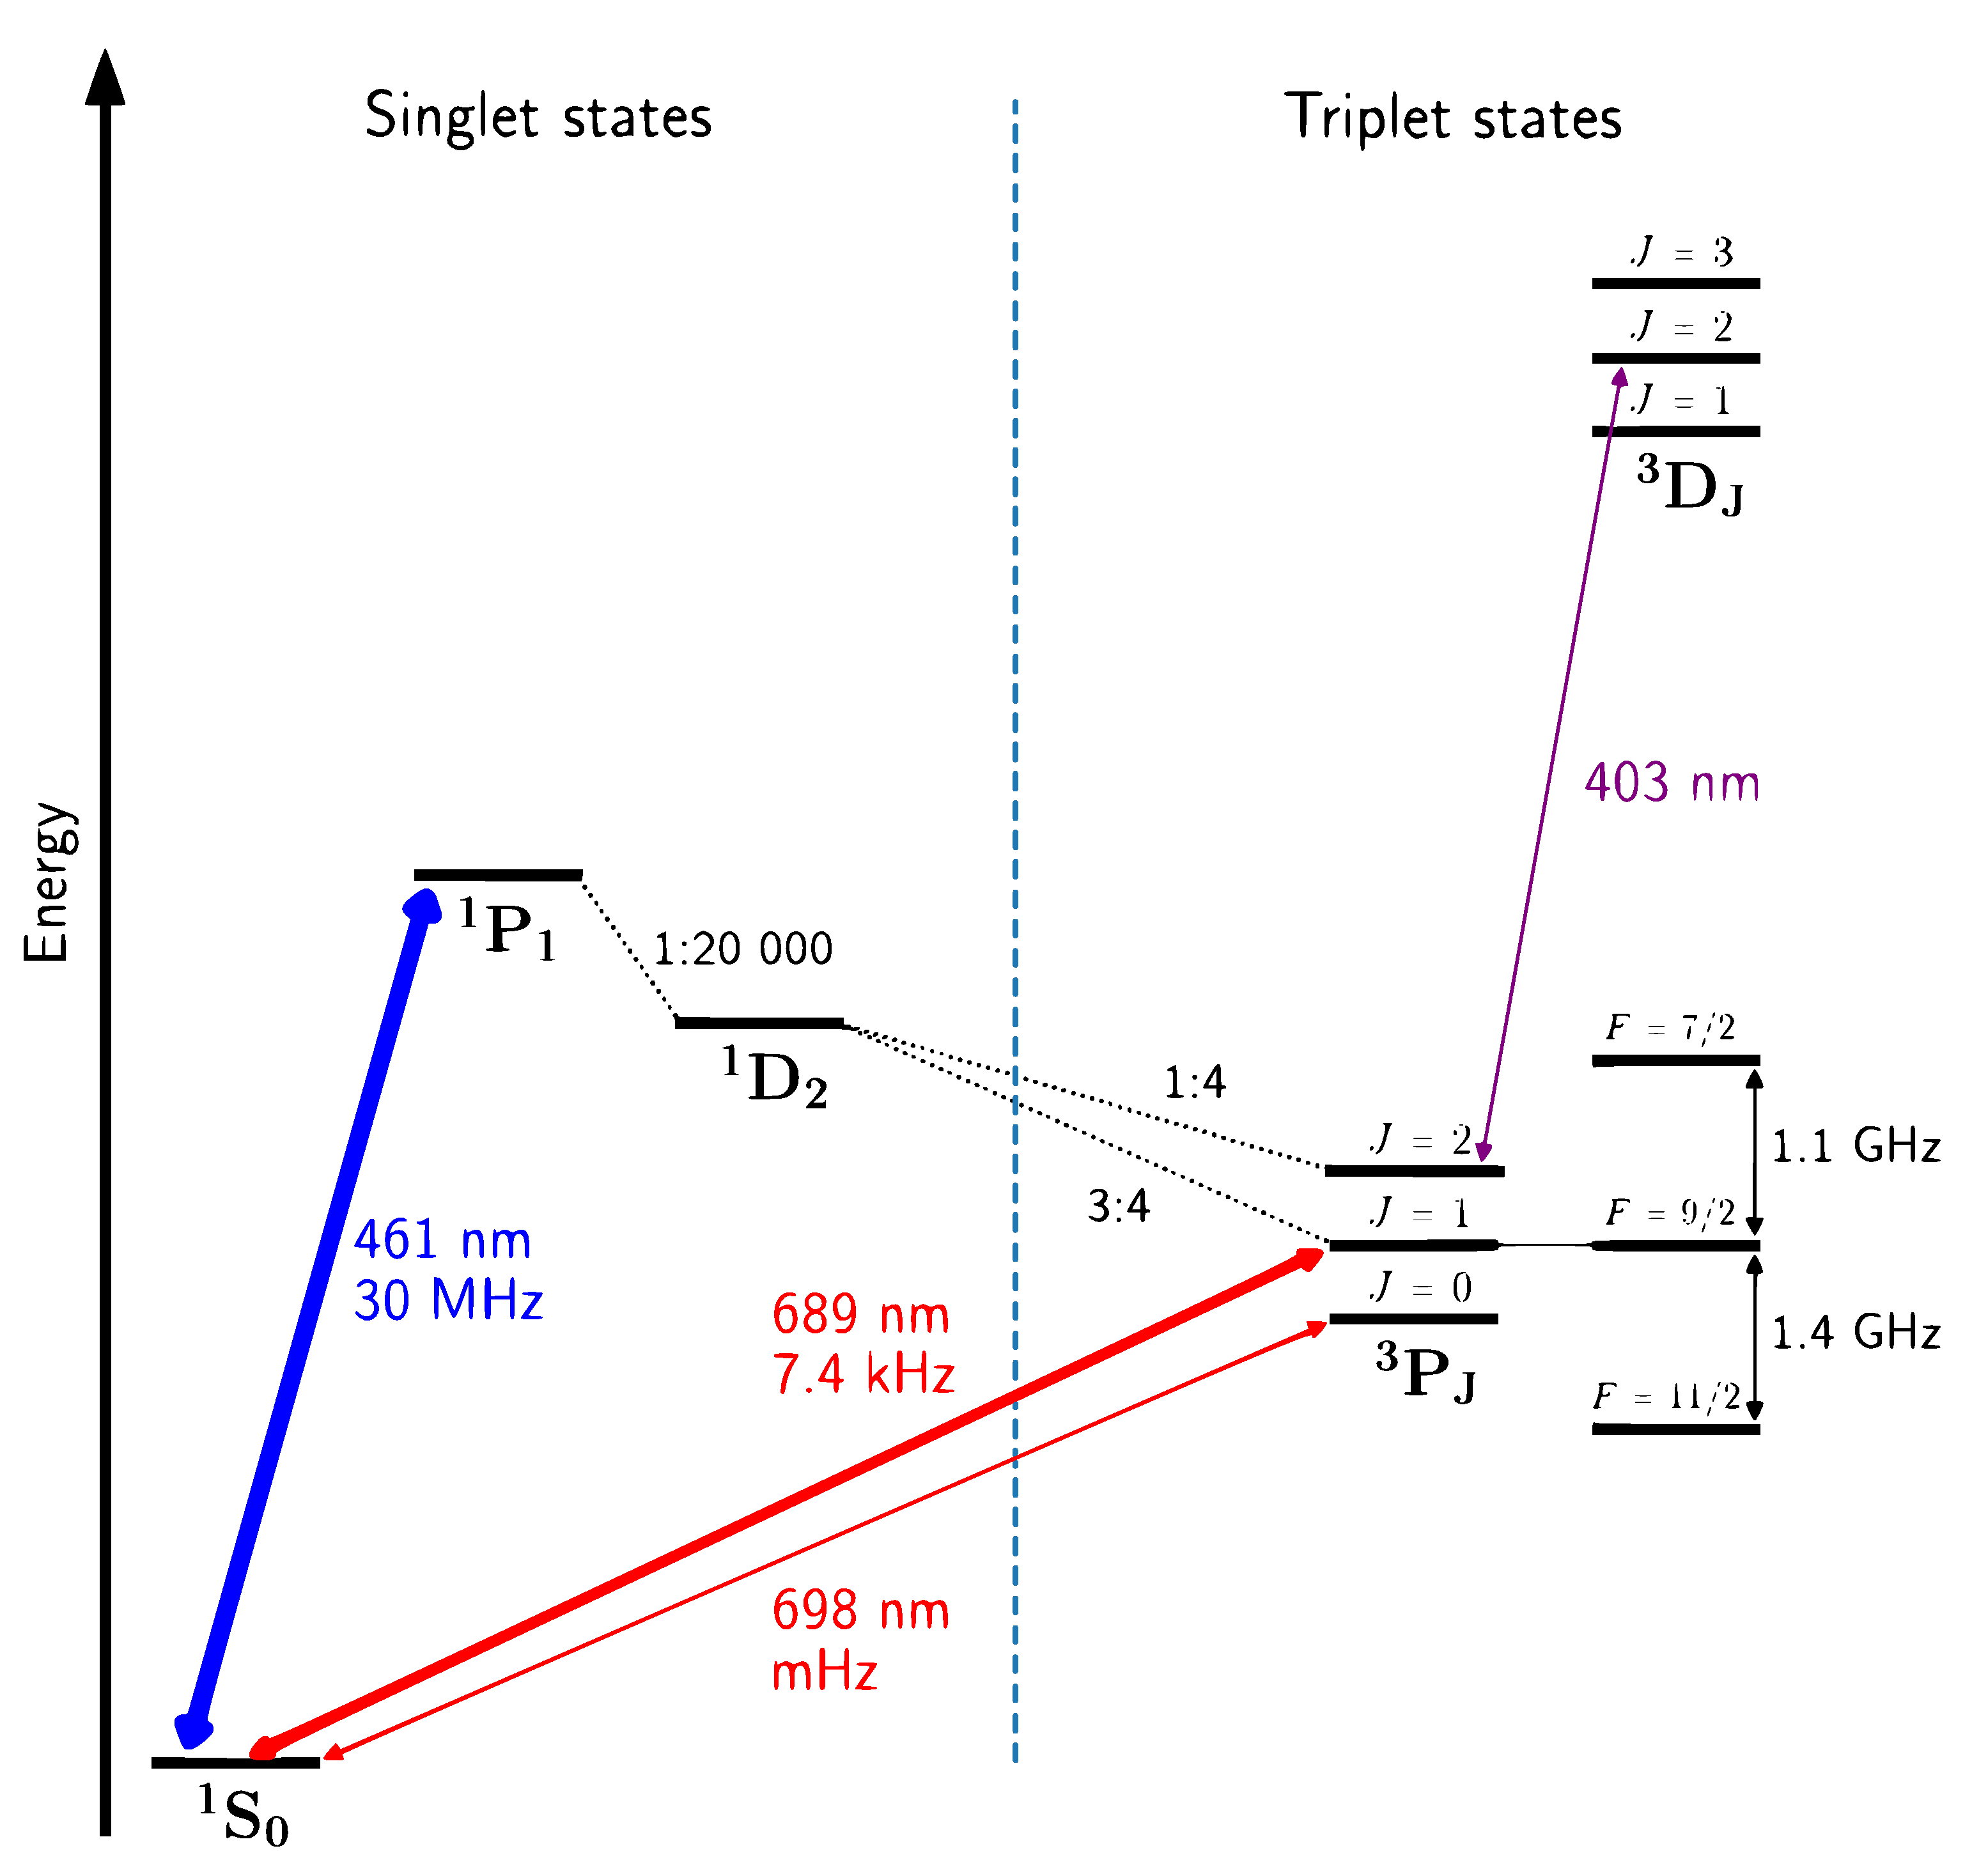
\includegraphics[width=1\linewidth]{Chapitres/Gas preparation and spin control/images/energy_levels_sr.pdf}
\caption[Energy diagram of $^{87}\text{Sr}$]{Extracted from \cite{litvinov_these} Energy spectrum of $^{87}\text{Sr}$ including fine and hyperfine interactions. In blue the $461~$nm transition used for TC, Zeeman cooling, blue MOT stage and imaging. The purple arrow indicates the repump line at $403~$nm from the metastable state $^3P_2$ used for the atoms leaking from the intermediate $^1D_2$ state. In red the transition to $^3P_1$ at $689~$nm used for all stages of the red MOT, optical pumping, spin manipulation, coherent manipulation (see Chap.\ref{chap 2}), photoassociation (see Chap.\ref{chap 3}, through
the different hyperfine states $F=7/2, 9/2, 11/2$).
The 698~nm transition indicates the clock transition which we do not use in this experiment.}
\label{energy levels sr}
\end{figure}

Fig \ref{setup exp} is a representation of the entire experimental setup that summarizes the speed of the atoms, real magnetic gradient, the temperature and the size of the gas for every cooling stage.

The complete timing sequence -- magnetic field ramps, laser intensities, and laser frequencies -- for every stage described in this chapter is summarized in
Fig.~\ref{fig:sequence_sr87}.


\begin{figure}[H]
    \centering
    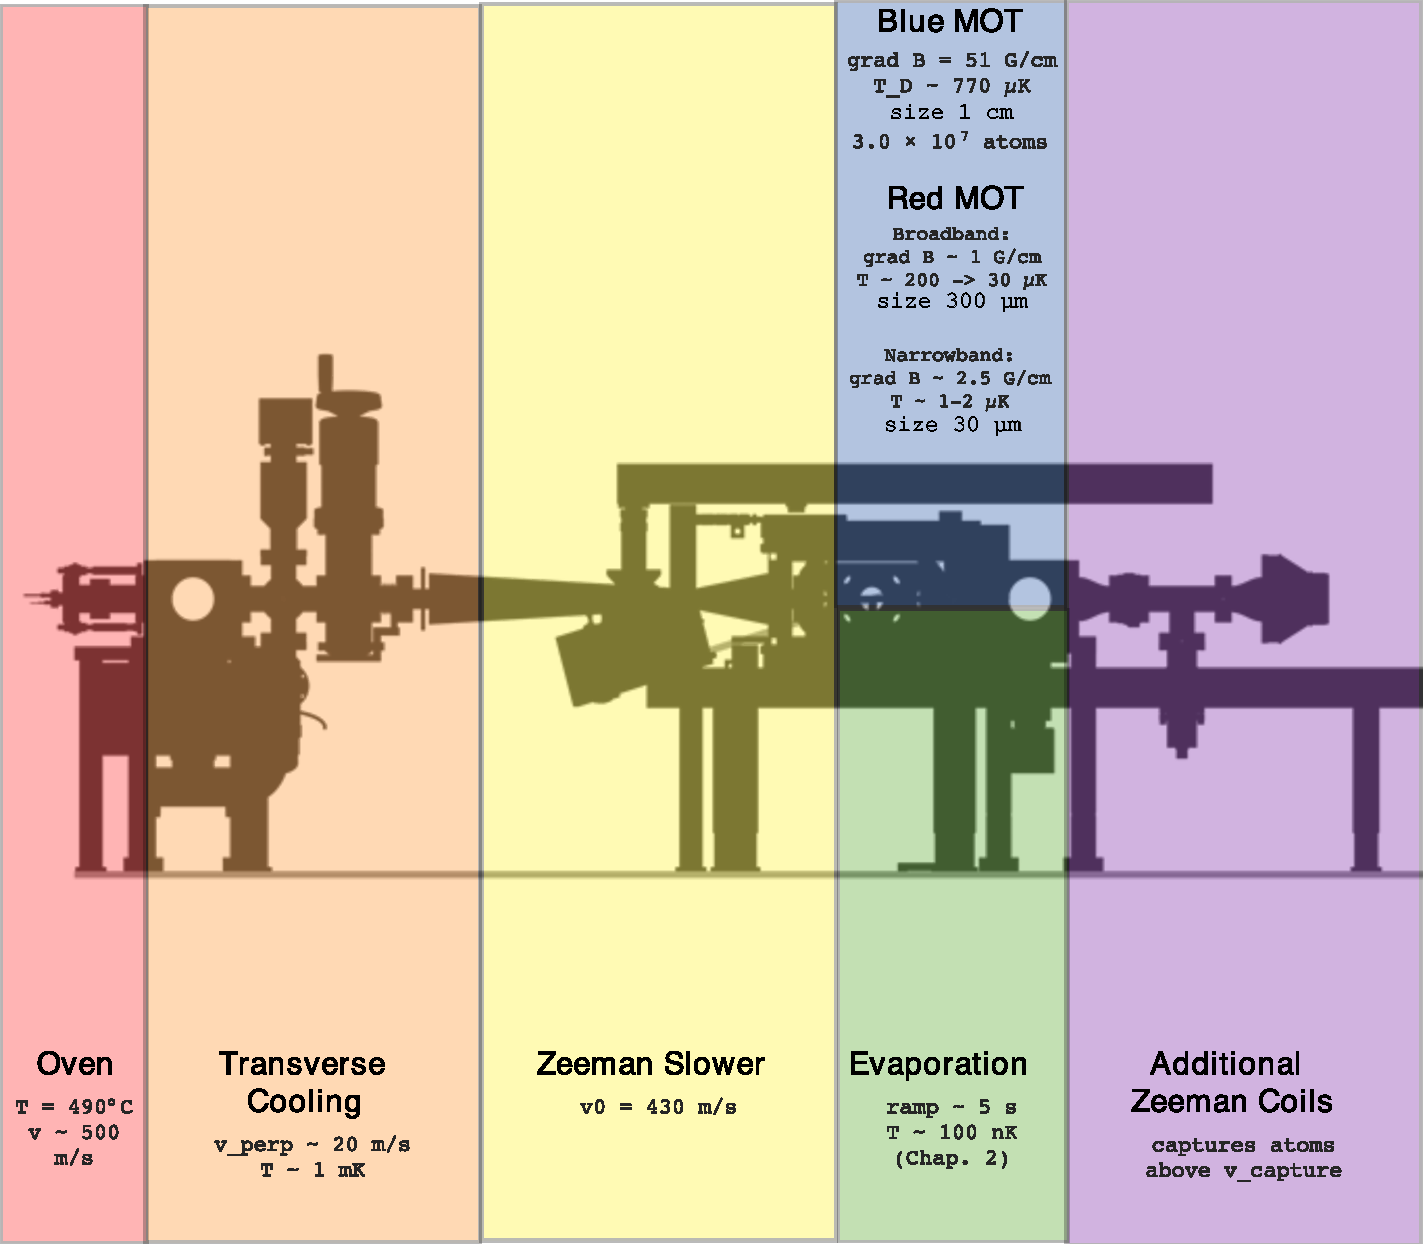
\includegraphics[width=1\linewidth]{Chapitres/Gas preparation and spin control/images/setup_exp.pdf}
    \caption{Extracted and modified from \cite{bataille_realisation_nodate} Experimental full setup for the cooling and trapping of the atoms with figures on the velocity, temperature and typical magnetic gradient on each stage.}
    \label{setup exp}
\end{figure}


\begin{sidewaysfigure}
    \centering
    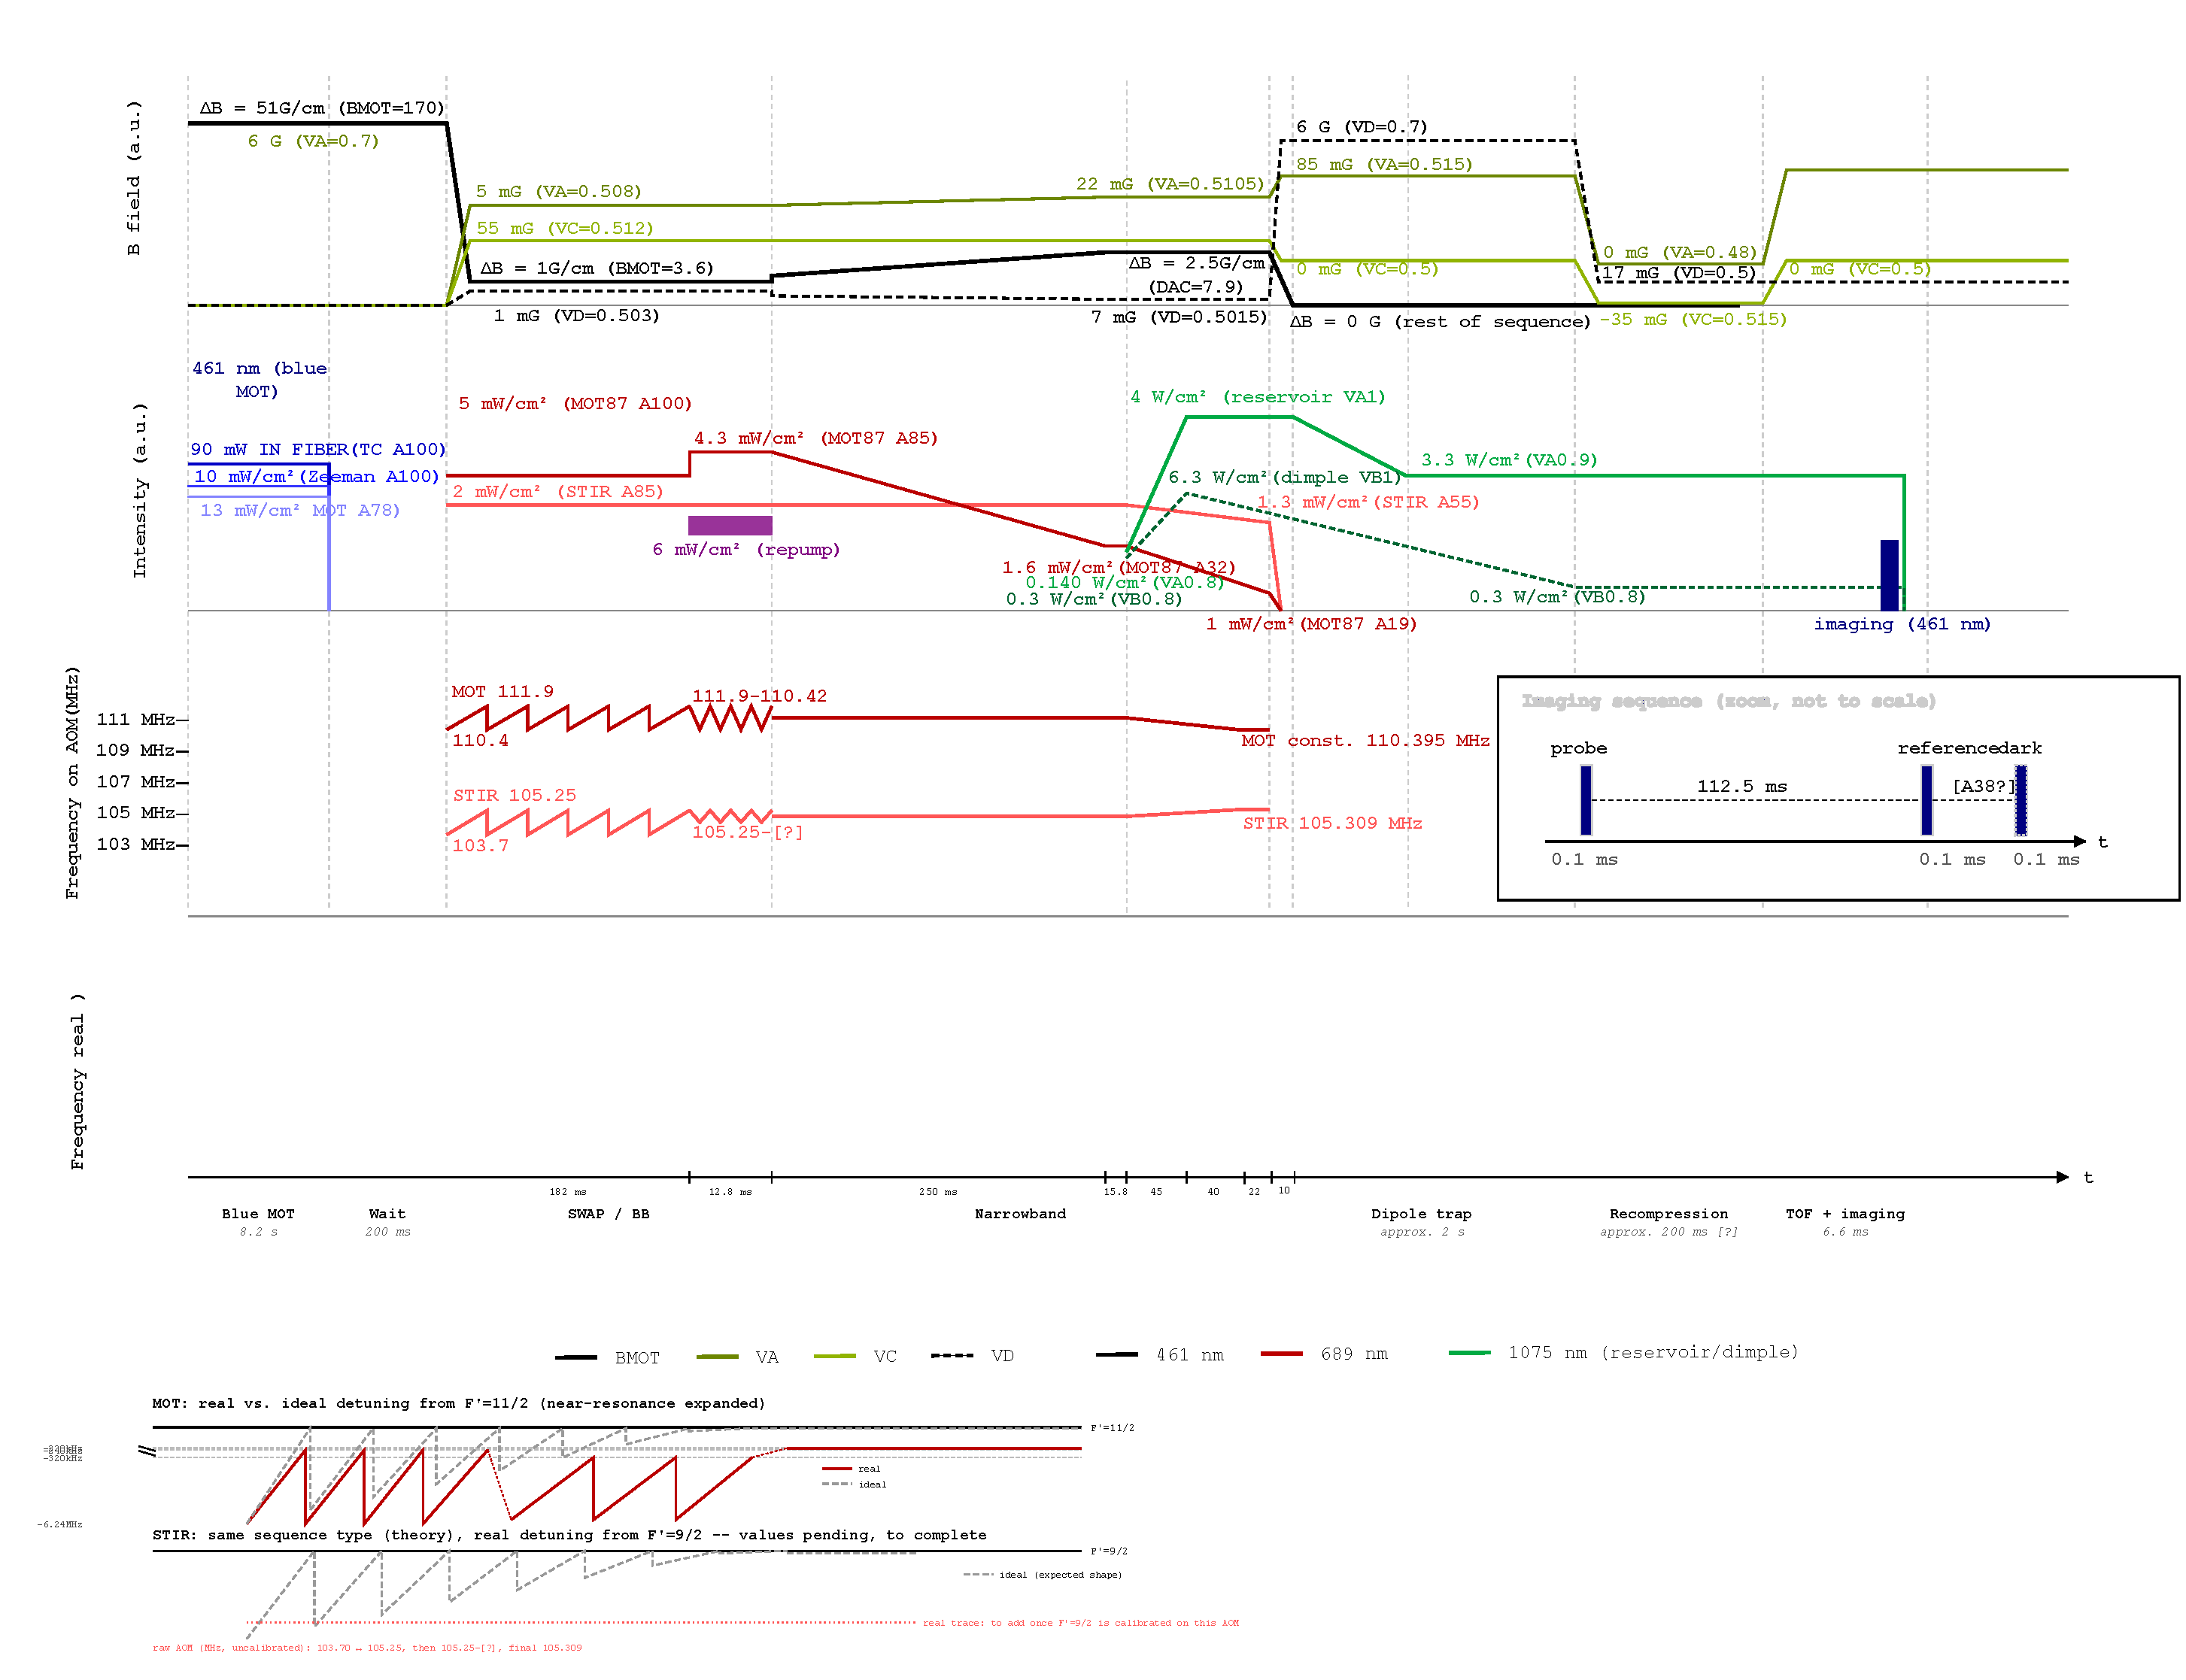
\includegraphics[width=\textheight]{Chapitres/Gas preparation and spin control/images/sequence_Sr87_final.pdf}
    \caption[Experimental sequence for the magnetic field, laser intensities, and laser frequencies]{Experimental sequence for the magnetic field, laser intensities, and laser frequencies as a function of time, spanning the blue MOT through to time-of-flight imaging. Indicated intensities
    are the mean intensity in each fiber of the cooling stage (e.g intensity in 1/3 of the MOT fibers). Both real physical values and instructions on the variable attenuator (VA,VC,VD, BMOT) and the frequencies on the AOM's are writen for the reader and the experimentators of this machine. 
    \textbf{Top:} magnetic field gradient (BMOT) and the three bias/compensation coil voltages (VA, VC, VD). \textbf{Middle:} intensities of the $461~$nm, $403~$nm, $689~$nm, and $1075~$nm light. \textbf{Bottom:} frequency detunings of the entire red cooling stages. Frequencies of 
    blue MOT, repumper and reservoir/dimple beams are not indicated since they do not change through the entire sequence. 
    The bottom right inset details the imaging sequence (probe, reference, and dark exposures).}
    \label{fig:sequence_sr87}
\end{sidewaysfigure}


\section{Fermi gas preparation}
\subsection{Blue optical setup}
Solid strontium is vaporized in an oven heated to $\textcolor{blue}{490}^\circ\text{C}$, outputting an atomic beam through a cluster of fine capillaries that provide initial spatial collimation.

The first cooling stages operate on the main $^1S_0 \rightarrow {}^1P_1$ transition using a master-slave laser architecture (see Fig.~\ref{fig:intro-chaine-bleue}). The master laser is an Extended-Cavity Diode Laser (ECDL, New Focus Vortex) frequency-stabilized via saturated absorption spectroscopy on $^{87}\text{Sr}$ \cite{bataille_realisation_nodate}. It seeds three high-power slave laser diodes, forcing them to inherit the master's narrow linewidth and central frequency while delivering the high output power needed for the cooling beams. 

\begin{figure}[H]
    \centering
    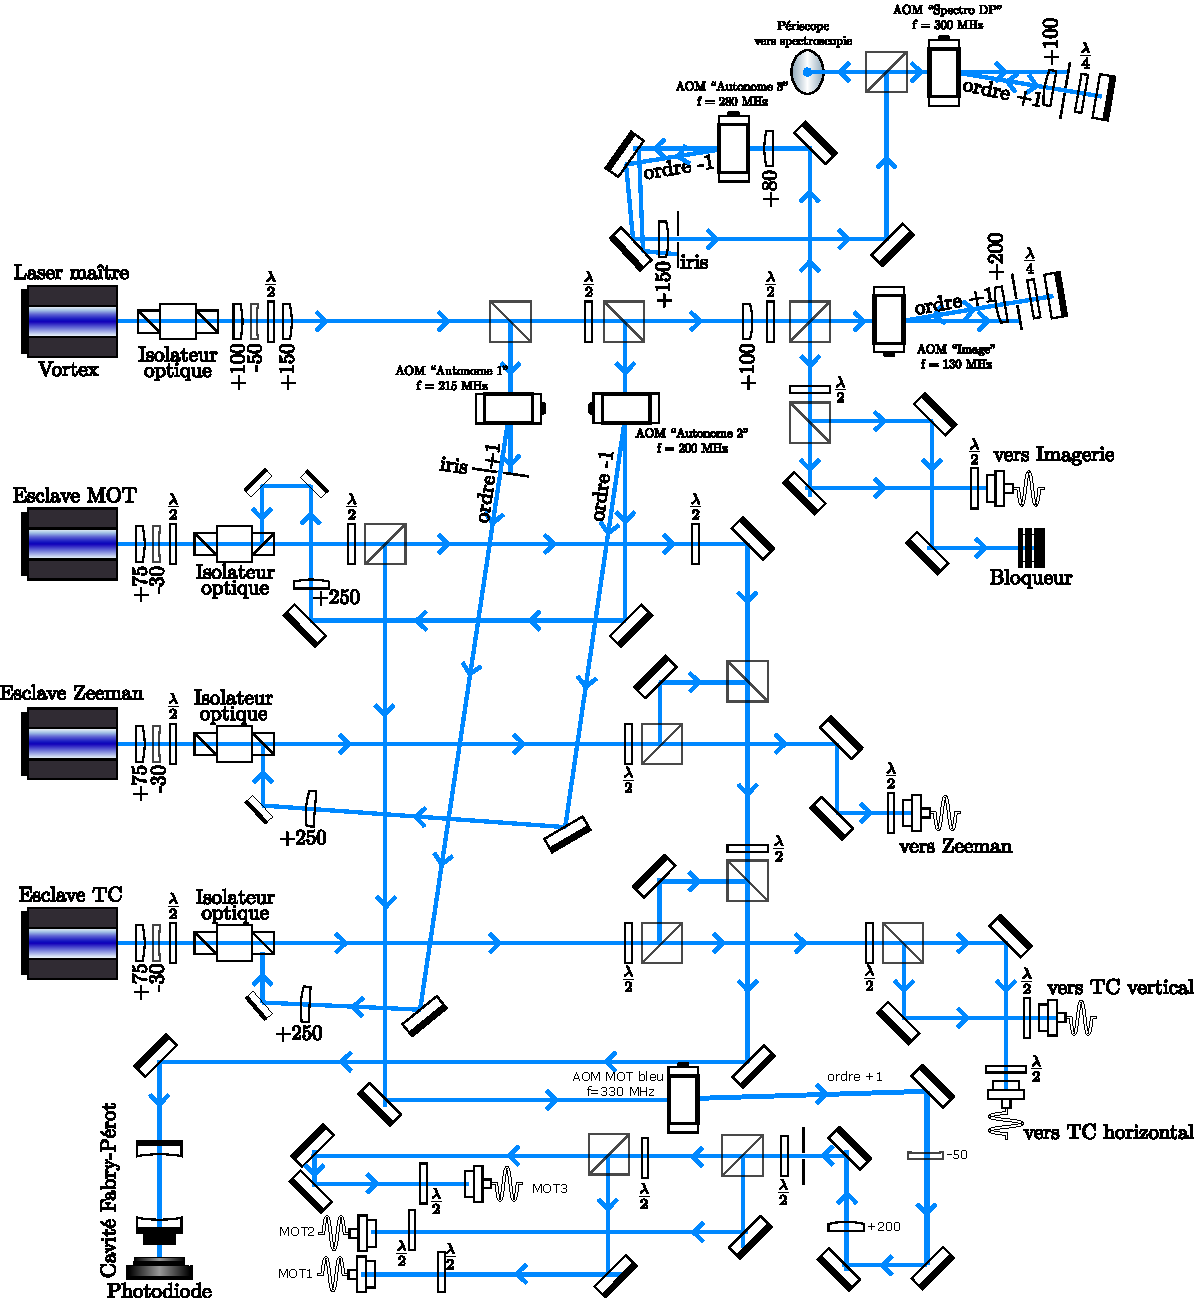
\includegraphics[width=1\linewidth]{Chapitres/Gas preparation and spin control/images/chaine_bleue_actualisée.pdf}
    \caption[Optical layout of the $461~\text{nm}$ blue laser system ]{Optical layout of the $461~\text{nm}$ blue laser system for transverse cooling, Zeeman slowing, and blue MOT.}
    \label{fig:intro-chaine-bleue}
\end{figure}

\begin{figure}
    \centering
    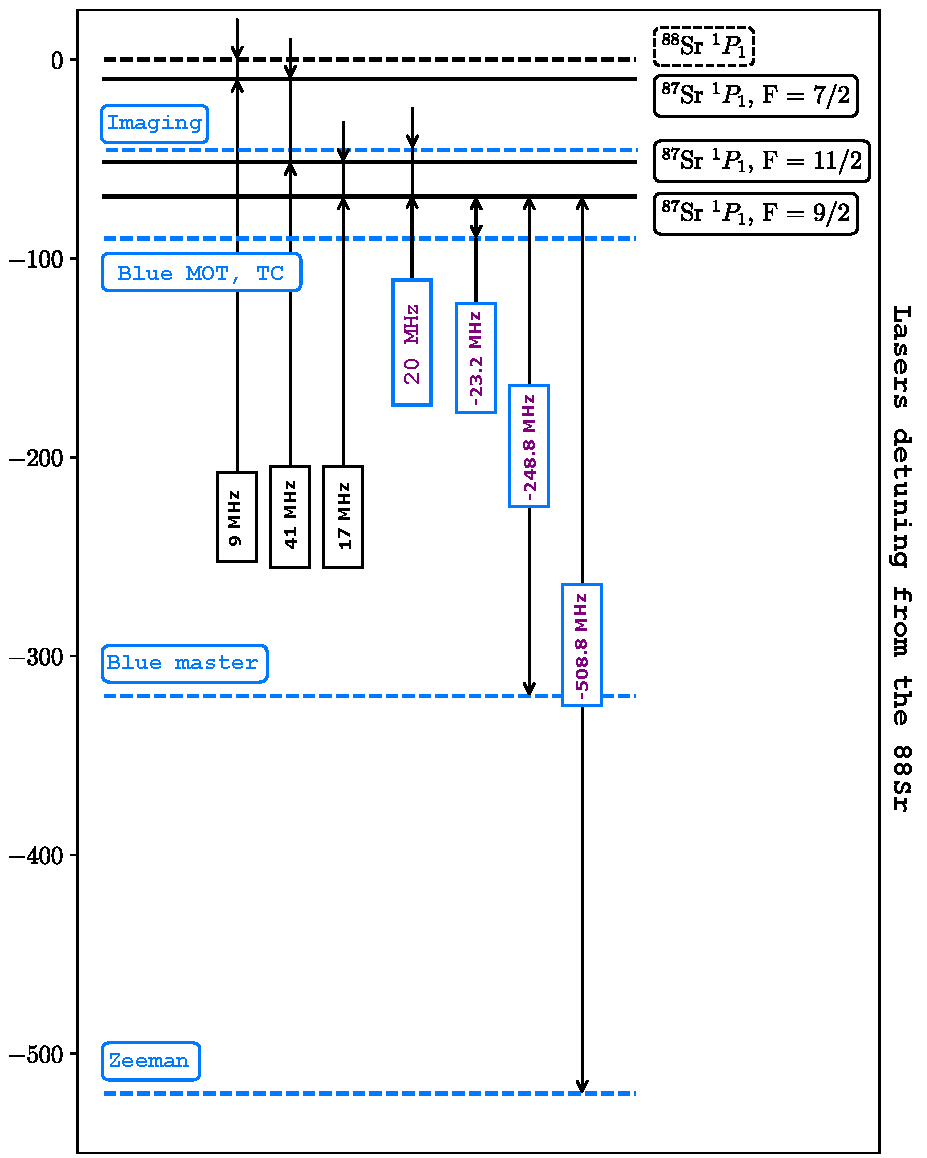
\includegraphics[width=1\linewidth]{Chapitres/Gas preparation and spin control/images/frequences_bleues.pdf}
    \caption[ Diagram of the frequencies of each laser composing the blue chain]{Adapted from P.Bataille thesis \cite{Bataille2020} Diagram of the frequencies of each laser composing the blue chain of the blue MOT broadband cooling. Blue dashed lines indicate the tunable frequencies of the lasers. Plain black lines indicate the transitions of \text{$^{87}Sr$ and $^{88}Sr$ isotopes. The 
    frequencies refer mostly to the optical frequency at the output of the laser called `Blue master'.}}
    \label{frequences bleues}
\end{figure}

\subsection{Transverse cooling}

Following extraction from the oven capillaries, the atomic beam is further collimated using 2D transverse cooling (TC). This stage employs two orthogonal pairs of counter-propagating laser beams perpendicular to the main longitudinal atomic propagation axis ($z$-axis), reducing the transverse velocity spread $v_\perp$ via photon recoil momentum ($\hbar k_\perp$).
The perpendicular velocity is reduce to about 20~m/s.

\subsubsection{Operating principle and radiation pressure}

The collimation relies on Doppler cooling. An atom moving with a transverse velocity $\vec{v}_\perp$ experiences a Doppler shift $\Delta_D = -\vec{k}_\perp \cdot \vec{v}_\perp$. As illustrated in Fig.~\ref{fig:doppler_shift}, atomic velocity classes observe shifted transition resonances centered at $\omega_0 \pm \vec{k}_\perp \cdot \vec{v}_\perp$. 
When the laser frequency is red-detuned ($\Delta < 0$) with respect to the atomic transition frequency ($\omega_0$, the center of the purple gaussian), the atom preferentially absorbs photons from the counter-propagating beam, generating a net damping force.

\begin{figure}[H]
\centering
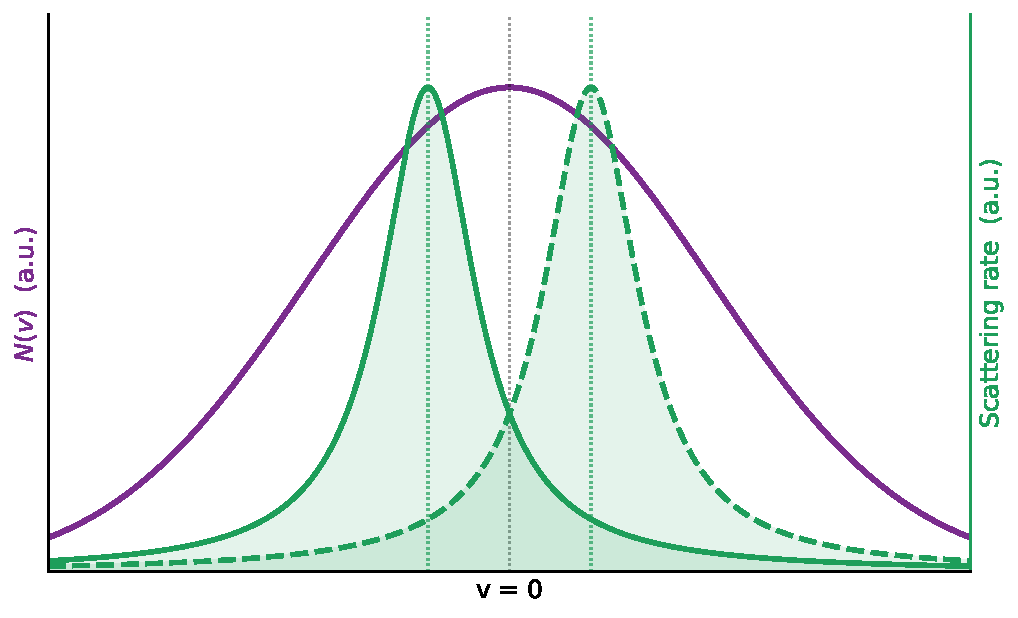
\includegraphics[width=1\linewidth]{Chapitres/Gas preparation and spin control/images/transverse_cooling_distribution.pdf}
\caption[Illustration of the transverse cooling effect]{Illustration of the transverse cooling effect on the atoms arriving from the oven spread in different velocity classes. }
\label{fig:doppler_shift}
\end{figure}

In the low-intensity limit ($s \ll 1$), standard Doppler cooling theory shows that the
equilibrium temperature $T(\Delta)$, set by the competition between the velocity-dependent
damping and the momentum diffusion from photon scattering, is minimized at a detuning of
$\Delta_{\text{eff}} = -\Gamma/2$, yielding the Doppler temperature limit
$T_D = \hbar\Gamma/(2k_B)$.

\subsubsection{Experimental setup and laser configuration}

For this stage, we drive the broad-linewidth $^1S_0 \rightarrow {}^1P_1$ transition ($\Gamma / 2\pi = 30.5~\text{MHz}$, $I_{\text{sat}} \approx 40~\text{mW/cm}^2$). The laser frequency $f_{\mathrm{TC}}$ is generated by shifting the main blue master frequency using an acousto-optic modulator (AOM) driven at $f^{\mathrm{RF}}_{\mathrm{TC}}$:
\begin{equation}
f_{\mathrm{TC}} = f_{\mathrm{Blue,Master}} + f^{\mathrm{RF}}_{\mathrm{TC}}
\end{equation}

The horizontal arm is operated at roughly three times the intensity of the vertical arm,
with $I/I_{\text{sat}} = 0.25$ in the horizontal arm: there is no physical reason why it is
this way but we observe the best cooling for this ratio. Both arms nonetheless remain
below saturation ($I < I_{\text{sat}}$) over an interaction area of approximately
$10~\text{cm}^2$. The TC laser remains active throughout the subsequent
blue-cooling stages to ensure continuous atomic-flux collimation.

\subsubsection{Detuning and power optimization}

While ideal two-level theory predicts an optimal detuning of $\Delta = -\Gamma/2$, experimental constraints alter this optimum:
\begin{itemize}
\item \textbf{Power limitations over large beam areas:} Operating near saturation ($I \sim I_{\text{sat}}$) would maximize the velocity capture range through power broadening and larger radiation pressure forces. 
However, illuminating the $10~\text{cm}^2$ interaction area at saturation would require over $400~\text{mW}$ of optical power. Consequently, the system operates in the low-intensity regime ($I \ll I_{\text{sat}}$).
\item \textbf{Optimal detuning shift:} Experimental characterization reported in F. Faisant's thesis \cite{faisant_building_2024} demonstrated that maximum collimation efficiency (measured by downstream atom yield) is achieved for low intensity at $\Delta = -\Gamma/4$ rather than $-\Gamma/2$, 
as shown in Fig.~\ref{felix faisant}. Indeed considering the residual random motion of the atoms modifies the expression
of the total average force: minimum temperature is reached for higher intensities. This plot also illustrates how the maximum atom number gain improves with total beam power.
\end{itemize}
Future upgrades in progress include replacing the current TC slave diode with a higher-power diode and re-optimizing $\Delta_{\text{eff}}$ to further enhance atom capture.\\
Following transverse collimation, the atomic beam enters the Zeeman slower stage along the main longitudinal axis.

\begin{figure}[H]
\centering
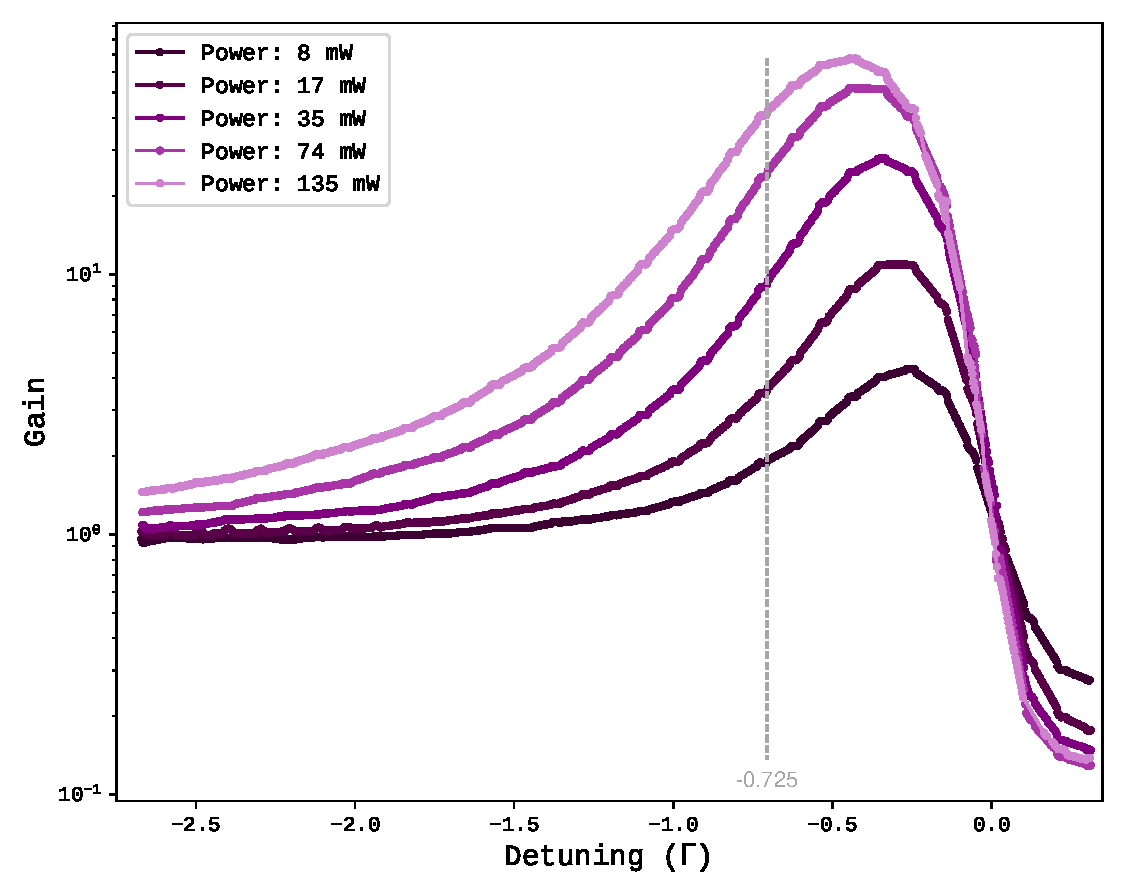
\includegraphics[width=0.8\linewidth]{Chapitres/Gas preparation and spin control/images/felix_faisant_these.pdf}
\caption[Discussion on TC detuning efficiency (Felix Faisant thesis)]{Transverse cooling performance as a function of laser detuning and power (adapted from \cite{faisant_building_2024}). Curves of atom number gain for different
optical powers on TC are showing optimum that are not centered on the same detuning.}
\label{felix faisant}
\end{figure}


\subsection{Zeeman cooling}
Following transverse collimation, atoms are decelerated longitudinally using a
Zeeman slower \cite{phillips_laser_1982}. The mechanism relies on a
counter-propagating laser beam maintained on resonance with the decelerating
atoms as they travel through a spatially varying magnetic field gradient $B(z)$
generated by a tapered solenoid.

To compensate for the decreasing Doppler shift $kv(z)$ as atoms slow down, the
magnetic field $B(z)$ shifts the Zeeman sub-levels to satisfy the resonance
condition along the entire deceleration path:
\begin{equation}
\Delta_{\text{eff}}(z) = \omega_{\text{laser}} - \omega_0 + k v(z) - \frac{\mu_B g_J B(z)}{\hbar} = 0
\label{eq:zeeman_resonance}
\end{equation}
Here, $\Delta_{\text{eff}}(z)$ is the local effective detuning experienced by the atom at position $z$; $\omega_{\text{laser}}$ and $\omega_0$ are the angular frequencies of the slowing laser and of the atomic transition, respectively; $k = 2\pi/\lambda$ is the laser wavevector; $v(z)$ is the atom's longitudinal velocity at position $z$; $\mu_B$ is the Bohr magneton; $g_J$ is the Land\'e factor of the excited electronic level; and $B(z)$ is the local magnetic field produced by the Zeeman slower.

Only atoms entering the slower with a velocity below the capture velocity
$v_0=430$~m/s can satisfy Eq.~\ref{eq:zeeman_resonance} and thus be decelerated;
faster atoms never come into resonance with the slowing beam and pass through
unaffected.

Solving Eq.~\ref{eq:zeeman_resonance} for the required field profile gives
\begin{equation}
B(z) = \frac{\hbar}{\mu_B g_J}\Big[k v(z) + \big(\omega_{\text{laser}} - \omega_0\big)\Big],
\label{eq:Bz_profile}
\end{equation}
with $\omega_{\text{laser}} - \omega_0 < 0$ (red-detuned laser) and $v(z)$
decreasing progressively along the slower. Whether $B(z)$ eventually changes sign
depends on the chosen detuning $|\omega_{\text{laser}}-\omega_0|$ relative to
$kv_f$, where $v_f$ is the target exit velocity: for
$|\omega_{\text{laser}}-\omega_0| > kv_f$, the field must cross zero and become
negative before the atoms reach $v_f$. 

Because the atom's direction of motion does not change, this sign change reflects
only the resonance condition of Eq.~\ref{eq:zeeman_resonance}, not a reversal of
the atomic trajectory: atoms continue to decelerate in the same direction
throughout. Supplementary coils of increasing radii, placed past this zero
crossing, produce the required negative field to keep the already-slowed atoms in
resonance down to the final capture velocity suitable for MOT trapping.

\subsection{Blue MOT}

The Magneto-Optical Trap (MOT) provides simultaneous spatial confinement and cooling. 

The blue MOT combines a magnetic quadrupole field (generated by anti-Helmholtz coils
centered on the vacuum chamber, driven at $170~\text{A}$ to produce a gradient of
$\Delta B = 51~\text{G/cm}$) with three orthogonal pairs of counter-propagating
$461~\text{nm}$ laser beams carrying opposite circular polarizations ($\sigma^+/\sigma^-$)
\cite{phillips_laser_1998}.

The position-dependent Zeeman shift lifts the degeneracy of the $m_F$ sub-levels:
\begin{equation}
\Delta E(z) = m_F\, g_F\, \mu_B\, B(z)
\end{equation}
Combined with the $\sigma^\pm$ polarization of the counter-propagating, red-detuned
beams, this position-dependent shift brings only one beam into resonance on either
side of the trap center ($z=0$), creating a restoring force toward $z=0$ alongside
the velocity-dependent radiation pressure force.
The vertical beam waist is twice smaller than the two horizontal one and the mean intensity 
of each axis is $I/I_{sat} = 0.3$ (13~mW/cm$^2)$.

During this stage, the cloud reaches the Doppler temperature limit \cite{dalibard_atomes_froids}:
\begin{equation}
k_B T_D = \frac{\hbar \Gamma_{^1S_0 \rightarrow {}^1P_1}}{2}
\end{equation}
Due to the broad linewidth of the $461~\text{nm}$ transition ($\Gamma/2\pi = 30.5~\text{MHz}$), this Doppler temperature ($T_D \approx 770~\mu\text{K}$) remains significantly higher than the single-photon recoil limit $T_r$.\\
The atoms are transfered in $^1P_1$ state that is determined by the equation evolution of the atom number:
\begin{equation}
    \frac{dN(t)}{dt} = \alpha \Phi -\gamma_{loss}N(t)
\end{equation}
where $\Phi$ is the incident atomic flux on the MOT capture region, $\alpha$ is the dimensionless capture efficiency (the fraction of that flux actually trapped, depending on experimental parameters), $\gamma_{loss} = \gamma_{vacuum} + \gamma_{leak}$ respectively the loss rate due to the imperfection of the vacuum and the rate leakage to the
metastable state. Then the number of atom in time evolves as:
\begin{equation}
    N(t) = N_{sat}(1-e^{-t/\tau})
\end{equation}
$N_{sat} = \alpha \Phi \tau$ when the transition reaches its maximum value. Since the blue MOT lifetime is dominated by the leak into the metastable state and amounts to a few tens of milliseconds \cite{stellmer_creation_2012}, saturating the blue MOT atom number only requires waiting for a few such lifetimes. \\

The experimental accumulation time, however, is set by a different consideration: reaching the maximum number of atoms trapped in the metastable state, which takes $8.2~\text{s}$. Although the blue-MOT population itself saturates within a few tens of milliseconds, only a fraction of the atoms leaking out of the $^1P_1$ cycle end up trapped in the long-lived metastable state on each pass -- the rest decay back to the ground state and re-enter the blue-MOT cycle, where they must leak again before being retained (see branching ratios below). Accumulating a large fraction of the atoms into the metastable reservoir therefore requires many such cycles, hence the much longer $8.2~\text{s}$ duration. Throughout this accumulation, the magnetic field gradient is kept at its maximum, acting as a magnetic trap that confines the atoms in the metastable state, whose magnetic dipole moment is non-zero.


\subsection{Repumper}

A repumping laser system recovers these accumulated atoms into the cooling cycle: of the roughly $1{:}20000$ photon-scattering events on $^1P_1$ that decay via $^1D_2$ rather than back to the ground state, about $1{:}4$ reach the long-lived $^3P_2$ state addressed here (lifetime $\tau \approx 500~\text{s}$), with the rest returning through $^3P_1$. Without repumping, atoms trapped in $^3P_2$ remain dark to the $461~\text{nm}$ light and are permanently lost from the cooling cycle.

\subsubsection{Hyperfine structure of Strontium-87}
Because fermionic $^{87}\text{Sr}$ possesses a nuclear spin $I = 9/2$, its electronic states exhibit a rich hyperfine structure that must be addressed for efficient repumping.

Repumping is provided by a $403~\text{nm}$ external-cavity diode laser (TOPTICA). To address multiple $F$ hyperfine sub-levels (see Fig.~\ref{fig:intro-energy-levels-repumper}), the laser frequency is rapidly swept over a 3~GHz bandwidth for 3.2~ms.

\begin{figure}[H]
    \centering
    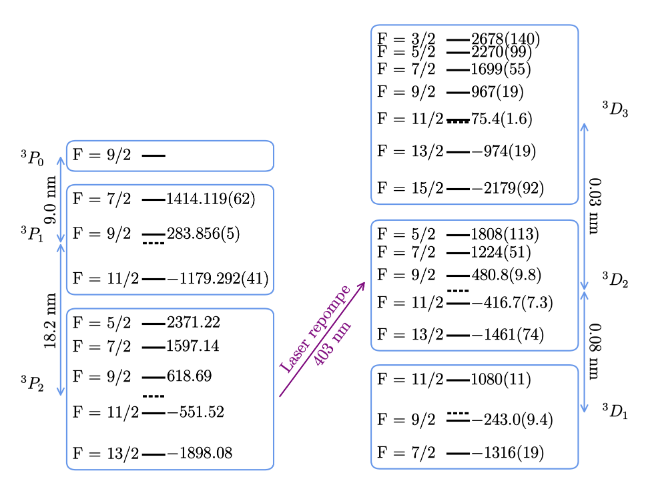
\includegraphics[width=0.7\linewidth]{Chapitres/Gas preparation and spin control/images/energy_levels_repumper.png}
    \caption[Energy level diagram of $^{87}\text{Sr}$, $^3P_2$ transition]{Energy level diagram of $^{87}\text{Sr}$ of the transition $^3P_2$ to the hyperfine states of the $^3D_J$
    at $403~\text{nm}$ cooling.}
    \label{fig:intro-energy-levels-repumper}
\end{figure}

\subsubsection{Optimization of the repumper sweep}
The $^3P_2$ hyperfine levels are unequally populated during blue MOT decay due to their differing $g_F$ Landé factors, affecting their magnetic trapping efficiency \cite{stellmer_creation_2012}.

To recover this population into the cooling cycle, the sequence proceeds as follows: the $461~\text{nm}$ beam is first extinguished at the end of the blue MOT phase, preventing recovered atoms from being re-excited and recycling back onto the blue transition; the $689~\text{nm}$ red MOT lasers are then switched on, so that atoms are captured as soon as they return to the ground state; finally, the $403~\text{nm}$ repumper is pulsed for $3.2~\text{ms}$ at $I\approx15~\text{mW/cm}^2$, starting $9.3~\text{ms}$ after the red MOT lasers are switched on, and the red MOT is left running afterwards. The repumper frequency is scanned over a range optimized around $3~\text{GHz}$ to selectively cover the $F=11/2$ and $F=13/2$ states; scanning a wider range would reduce total atom recovery by decreasing the dwell time on these critical transitions.

\begin{figure}[H]
    \centering
    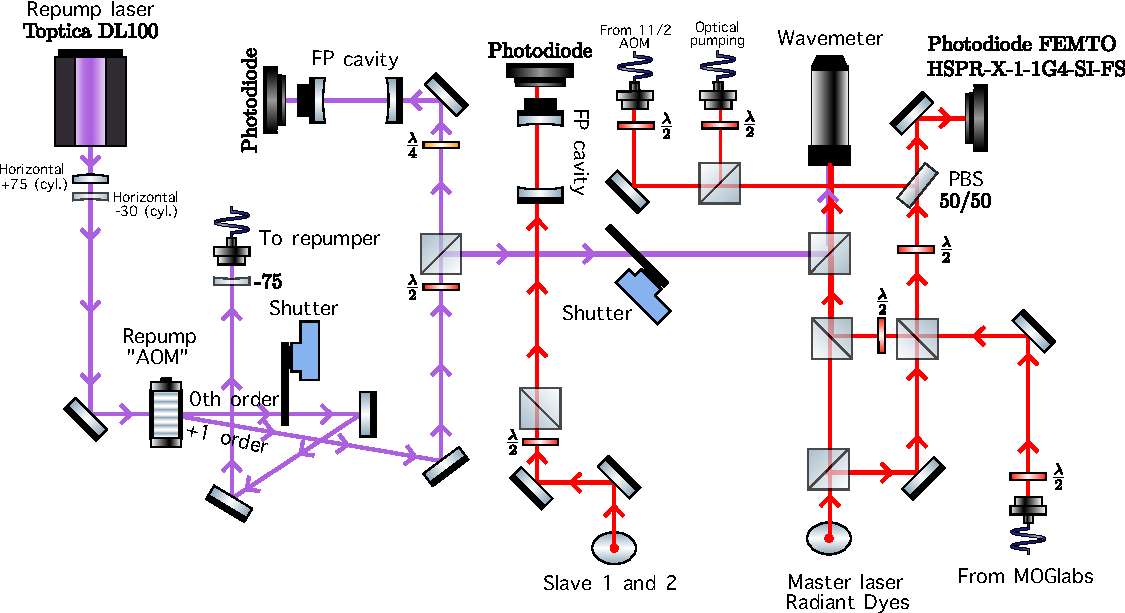
\includegraphics[width=1\linewidth]{Chapitres/Gas preparation and spin control/images/table_repumper.pdf}
    \caption{Optical setup for the repump and the beat-lock setup of the MOGlabs laser onto the Radiant Dyes.}
    \label{fig:intro-repompeur}
\end{figure}

\subsection{Laser cooling on the intercombination line : the ``red MOT''}

\subsubsection{Optical setup}
Because the blue MOT temperature is bounded by $T_D \approx 770~\mu\text{K}$, further cooling requires transferring atoms to the narrow intercombination transition $^1S_0 \rightarrow {}^3P_1$ at $689~\text{nm}$ ($\Gamma = 2\pi \times 7.4~\text{kHz}$).

For this transition, the formal Doppler limit ($T_D = \hbar \Gamma / m k_B = 177~\text{nK}$) falls below the single-photon recoil limit ($T_r = \hbar^2 k^2 / 2m = 462~\text{nK}$). Consequently, the ultimate red MOT temperature is bounded by the photon recoil limit.

The $689~\text{nm}$ light is generated by a commercial laser locked to an ultra-stable optical cavity refered as ``Red lock'' in Fig.\ref{frequences rouges} that contains all the frequencies of the red chain. The red master laser, from which the MOT, STIR, and optical pumping beams are all derived, has an optical frequency -220~MHz detuned from the $^{88}Sr, ^3P_1$. The `Red lock' is 
the summation of the 'AOM Inj Slave 1' that enables to access GHz away transitions from the bosonic state, with the RF frequency of the ultrastable cavity AOM.

Double-pass AOMs then fine-tune the frequency of MOT and Stir beams individually before splitting into three spatial counter-propagating beam pairs, bringing the actual atom-light detuning down to the much smaller values used for trapping (see below).

\begin{figure}
    \centering
    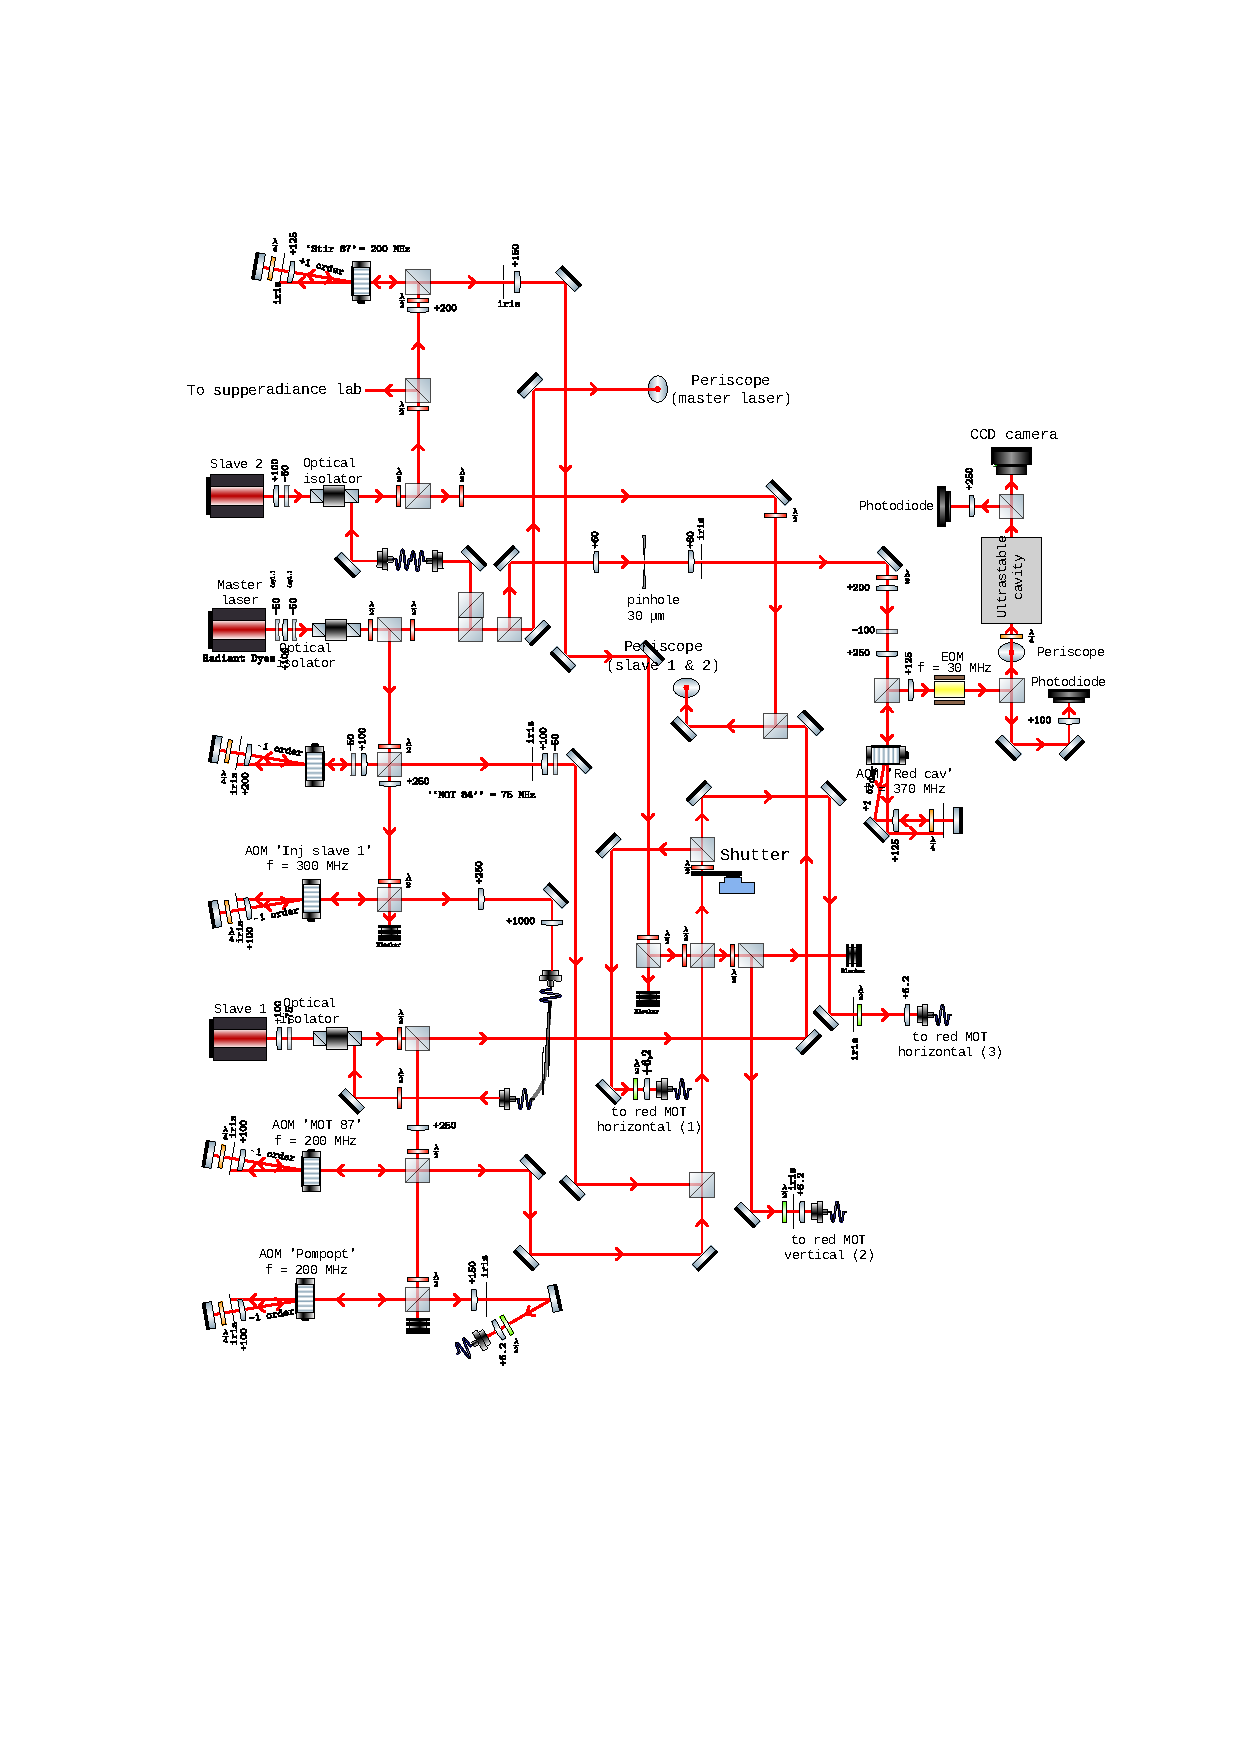
\includegraphics[width=1\linewidth]{Chapitres/Gas preparation and spin control/images/table_rouge.pdf}
    \caption{Optical setup of the $689~\text{nm}$ laser cooling system.}
    \label{fig:intro-chaine-rouge}
\end{figure}


\begin{figure}
    \centering
    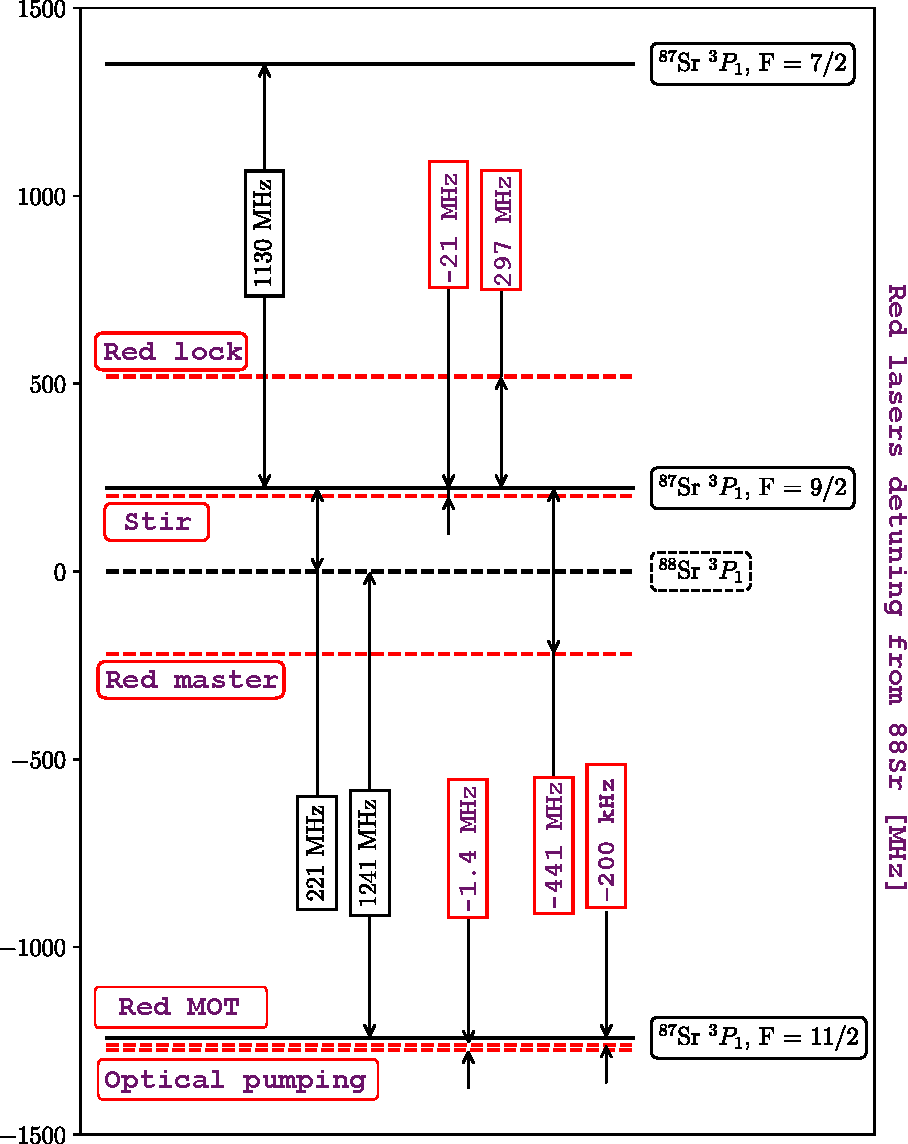
\includegraphics[width=1\linewidth]{Chapitres/Gas preparation and spin control/images/LevelDiagramRed.pdf}
    \caption[Frequencies of the red lasers used for the red MOT cooling stages]{Frequencies of the red lasers used for the red MOT cooling stages and optical pumping. The red dashed lines correspond to the tunable frequencies, the dark plain lines for the $^{87}Sr$ hyperfine states of transition $^3P_J$ and the $^{88}Sr$}
    \label{frequences rouges}
\end{figure}

\subsubsection{Broadband MOT}
At the end of the blue MOT, approximately $30$ million atoms have been captured; their
spatial spread ($ \simeq 300~\mu\text{m}$, reached at the end of the SWAP stage)
and thermal energy exceed the capture velocity of a single-frequency $689~\text{nm}$
MOT. To capture these thermal atoms, a broadband MOT is implemented on the
$^1S_0\,(F=9/2) \rightarrow {}^3P_1\,(F=11/2)$ transition under a weak magnetic field
gradient ($\Delta B \simeq 1~\text{G/cm}$, bias coil voltage VA = 0.50), operated in
two successive stages.

In the first stage, lasting $182~\text{ms}$, SWAP (Sawtooth Wave Adiabatic Passage) cooling is applied
\cite{bartolotta_laser_2018}. Two counter-propagating beams have their frequency swept
slowly and linearly through resonance, then reset almost instantaneously back to the start
of the ramp. The slow ramp is adiabatic and drives two sequential, stimulated transfers --
absorption from the beam the atom is moving towards, followed by emission into the
opposing beam, their Doppler shifts setting the time ordering -- removing $2\hbar k$ of
momentum per sweep without relying on spontaneous emission. The fast reset, in contrast,
is deliberately non-adiabatic so that it drives no transfer, and hence no momentum kick,
back the other way; a symmetric ramp would instead undo the cooling just achieved. The
trapping beam (MOT) is swept between $111.9$ and $110.4~\text{MHz}$ -- corresponding to a
real detuning from the $^3P_1\,(F'=11/2)$ resonance (calibrated at $110.34~\text{MHz}$ on
this AOM) of $-6.24~\text{MHz}$ to $-240~\text{kHz}$ -- while the stirring
beam (STIR, see below) is swept between $105.25$ and $103.7~\text{MHz}$
\textcolor{red}{\textbf{[TODO: convert to real detuning from $F'=9/2$ once its resonance
is measured on this AOM]}}, both starting at
an intensity of $I_{A100}(MOT87) = 5~mW/cm^2$ and $I_{A100}(STIR) = 2~mW/cm^2$. After $9.3~\text{ms}$, the repumper pulse
described above interrupts the STIR sweep for $3.2~\text{ms}$; the MOT and STIR sweeps then
resume for the remainder of the $182~\text{ms}$ stage. As the cloud cools and compresses
during this stage, the modulation amplitude $\Delta f$ is progressively ramped down together
with the optical power, which reaches $I_{A85} = 4.3~mW/cm^2$ for the MOT beam and
still $I_{A85} = 2~mW/cm^2$ for the STIR beam by the end of the stage. This process is
illustrated by the scheme of Fig.~\ref{fig:intro-red-mot-3-steps}, which represents the
total electronic spin projection as a function of B and position, with the bottom panel 
that corresponds to the actual frequency ramp in time. In the top figures dots on the 
Zeeman states indicates in black the states adressed at $t_0$ of the rampes, and in orange
the ones adressed by the frequency at $t_1$.

In principle, since SWAP relies on an adiabatic passage through resonance to generate a
deterministic momentum kick on every sweep, the detuning should start blue of resonance,
cross it, and end red-detuned by an amount that itself shrinks stage after stage as the
cloud cools further. In practice, however, the implemented sweep range given above
($-6.24$ to $-240~\text{kHz}$) remained entirely red-detuned relative to the $F'=11/2$
resonance and never actually crossed it -- indicating that this parameter was not fully
optimized (already represented in the sequence scheme \ref{fig:sequence_sr87}).

In the second stage, lasting $250~\text{ms}$ and visible on the right of
Fig.~\ref{fig:intro-red-mot-3-steps}, the cooling light is modulated with a conventional
sawtooth ramp detuned from resonance -- no longer swept symmetrically through it --
operating as a standard frequency-modulated Doppler-cooling MOT that further compresses
and cools the now colder, denser cloud. The MOT and STIR frequencies are ramped to their
narrowband values of $110.395~\text{MHz}$ (a real detuning of $-220~\text{kHz}$ from the
$F'=11/2$ resonance, measured after the slight magnetic-field adjustment described below)
and $105.309~\text{MHz}$ respectively
\textcolor{red}{\textbf{[TODO: STIR real detuning from $F'=9/2$, and the missing lower
bound of the stage-2 STIR ramp, to be added]}}, while the
bias coil voltage is raised to $V_C = 0.51$. Over this stage, the optical power is reduced
further, in two additional steps for the MOT beam -- from $I_{A85} = 2~mW/cm^2$, through
$I_{A32} = 1.6~mW/cm^2$, down to a final value of $I_{A19} = 1~mW/cm^2$ -- while the STIR
beam is reduced from $I_{A85} = 2~mW/cm^2$ to a final value of $I_{A55} = 1.3~mW/cm^2$.
By the end of this second stage, the cloud has cooled to an average temperature of
$T \simeq 30~\mu\text{K}$ with a size of $\simeq 300~\mu$m.

\subsubsection{Stirring laser}
The $\sigma^+/\sigma^-$ configuration of the red MOT introduces an intrinsic loss
channel arising from the large differential Land\'e $g$-factor between the ground
$^1S_0, F=9/2$ and excited $^3P_1, F'=11/2$ hyperfine levels. As illustrated in
Fig.~\ref{fig:intro-need-for-stir}, the position-dependent Zeeman shift
($B \sim x$) brings the two counter-propagating beams into resonance with
different $m_F'$ sub-levels at the same position: the $\sigma^+$ beam (green)
addresses the closed transition $m_F=9/2 \rightarrow m_F'=11/2$, while,
within the same laser linewidth (grey band), the $\sigma^-$ beam (purple)
simultaneously becomes resonant with the neighbouring, open transition
$m_F=9/2 \rightarrow m_F'=7/2$. This dual resonance is not by itself a loss
mechanism: the relative probability of the two processes, set by their
Clebsch-Gordan coefficients, favors the restoring transition by a ratio as
high as 55:1 in the most extreme case, so that the force averaged over many
scattering events remains restoring \cite{stellmerThesis}.

\begin{figure}[H]
\centering
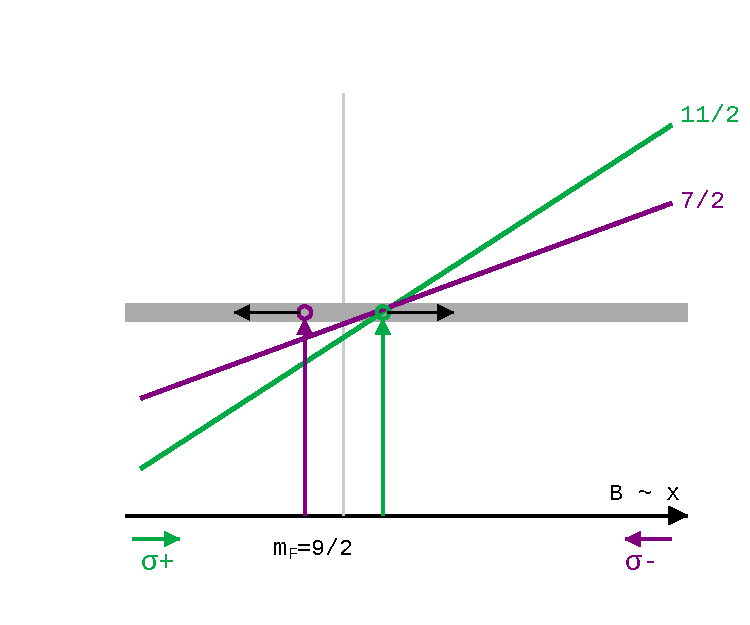
\includegraphics[width=0.8\linewidth]{Chapitres/Gas preparation and spin control/images/need_for_stir.pdf}
\caption[Illustration of the MOT effect on the $m_F$ states of the hyperfine $^3P_1,
F=11/2$ level]{(Adapted from \cite{stellmerThesis}) Illustration of the MOT effect on the $m_F$ states of the hyperfine $^3P_1,
F=11/2$ level. The position-dependent Zeeman shift brings the two counter-propagating
beams into resonance with different $m_F'$ sub-levels ($\sigma^+$ with the closed
transition to $m_F'=11/2$, $\sigma^-$ with the open transition to $m_F'=7/2$) at the same
position. The imbalance between the two processes, set by their Clebsch-Gordan
coefficients, still favors restoring trapping locally (see text); the actual loss
mechanism is discussed below.}
\label{fig:intro-need-for-stir}
\end{figure}

The condition for stable operation of a $F\to F+1$ MOT transition requires the
double inequality $F/(F+1) < g_e/g_g < F/(F-1)$ to hold \cite{stellmerThesis}.
For $^{87}$Sr, where $g_e/g_g\sim10^3$ due to the near-vanishing nuclear
magnetic moment of the $^1S_0$ ground state, this condition is violated by
several orders of magnitude. As a consequence, the resonance condition
$(m_F'g_e-m_Fg_g)\mu_B B(x) = h\Delta$ has a widely $m_F$-dependent slope:
low-$|m_F|$ states cross the laser resonance window (grey band) over a broad
range of positions, while the most Zeeman-shifted states cross it almost
vertically, remaining within resonance over such a narrow range of $x$ that
they are, in practice, essentially unaddressed by a fixed-frequency beam
(Fig.~\ref{fig:intro-randomisation}, left panel, akin to Fig.~2.8(d) of
\cite{stellmerThesis}).

The actual loss mechanism therefore appears when an atom finds itself on the
\emph{wrong} side of the trap for its $m_F$ state. There, neither beam can
come into resonance with it at all: the restoring force for an atom in
$m_F=9/2$ is maximal on one side of the trap only, and on the other side this
atom is lost from the trap entirely \cite{stellmerThesis}. This is especially
detrimental for the stretched states $m_F=\pm9/2$, whose cycling transition
is \emph{closed} and which therefore have no spontaneous decay path to
another $m_F$ state that could rescue them once on the wrong side.

A dedicated stirring laser mitigates this geometric loss by driving the open
$^1S_0 (F=9/2) \rightarrow {}^3P_1 (F=9/2)$ transition, superimposed on the
trapping light and red-detuned such that its resonance region overlaps with
that of the trapping transition (Fig.~\ref{fig:intro-randomisation}, left
panel, akin to Fig.~2.8(d) of \cite{stellmerThesis}). Because the differential
Zeeman shift of $F'=9/2$ is about five times smaller than that of $F'=11/2$
\cite{stellmerThesis}, driving this transition changes both where and how
broadly each $m_F$ state can come into resonance: the resonance position
shifts, potentially restoring resonance for atoms otherwise stuck on the
wrong side of the trap, and the resonance region in $x$ broadens by the same
factor, making it far more likely that an atom actually scatters enough
photons near resonance to be redistributed before drifting away. Since this
$F'=9/2$ transition is open, each excitation-decay cycle can additionally
redistribute the atom into a different $m_F$ sub-level of the ground state.

In our implementation, we additionally sweep the stirring laser's frequency
in a sawtooth pattern over time (Fig.~\ref{fig:intro-randomisation}, right
panel): at any instant, the fixed instantaneous frequency is simultaneously
resonant with several $(m_F, x)$ pairs across the trap (left panel), and as
the frequency sweeps, the ground-state $m_F$ population is continuously and
randomly redistributed. This continuous optical pumping brings atoms that
would otherwise remain trapped in an unfavorable $m_F$ state on the wrong
side of the trap back within reach of the cycling transition, restoring
efficiency to the cooling cycle.

\begin{figure}[H]
\centering
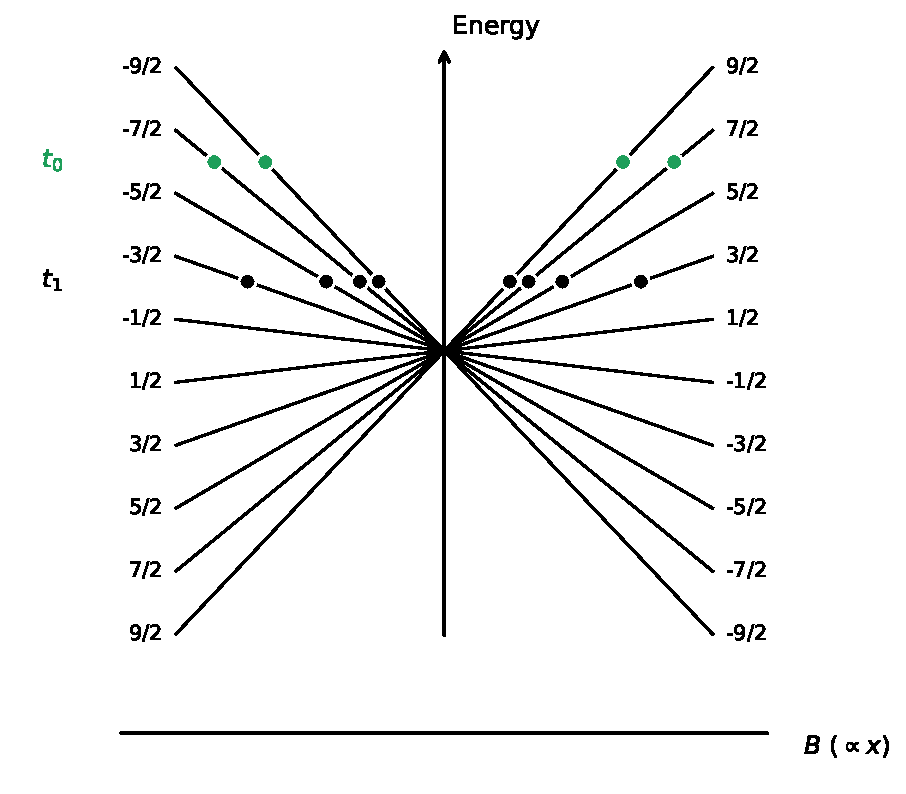
\includegraphics[width=0.95\linewidth]{Chapitres/Gas preparation and spin control/images/spin_randomization.pdf}
\caption[Illustration of the melange concept on the $^1S_0(F=9/2) \rightarrow
{}^3P_1(F=9/2)$ transition]{Spatial dependence of the resonance condition
on each $m_F$ sub-level, as a function of position $x$ ($B\propto x$) --
adapted from the principle illustrated in Fig.~2.8(d) of \cite{stellmerThesis}.
Right: the stirring laser's frequency, swept in a sawtooth pattern
\textit{over time} in our implementation. At each instant $t_0$, the
instantaneous frequency (right) is simultaneously resonant with several
$(m_F,x)$ pairs (left, black dots); sweeping this frequency over time thus
randomizes the $m_F$ population across the whole trap.}
\label{fig:intro-randomisation}
\end{figure}

While the broadened resonance region alone increases the fraction of the trap
addressed by the stirring light at any given detuning, a single, fixed
stirring frequency still only brings each $m_F$ state into resonance over a
finite, localized range of positions around its own resonance point
$x_{\text{res}}(m_F)$. An atom in a given $m_F$ state located outside this
window at a given time is simply not addressed, and nothing guarantees that
its thermal motion within the trap will ever bring it there. In our
implementation, we therefore additionally sweep the stirring laser's
frequency in a sawtooth pattern over time (Fig.~\ref{fig:intro-randomisation},
right panel): as the frequency ramps, the resonance position
$x_{\text{res}}(m_F,t)$ for each $m_F$ sweeps continuously across the trap,
so that every $m_F$ state is brought into resonance at every position over
the course of one ramp. This guarantees full coverage of the $(m_F,x)$ phase
space, rather than relying on the atom's own motion to bring it within reach
of a fixed, broadened resonance window.

\subsubsection{Narrowband MOT (Single-frequency MOT)}
Once the cloud is sufficiently cold, frequency modulation is switched off to operate a
single-frequency (monofrequency) MOT during a magnetic field ramp to $V_D = 0.70$
($\Delta B \simeq 2.5~\text{G/cm}$). This
stage reduces the temperature to $1\text{--}2~\mu\text{K}$ (near the recoil limit) with a
peak density of $n \simeq 10^8~$at/cm$^3$ and a size of 30~$\mu$m.
\begin{figure}[H]
    \centering
    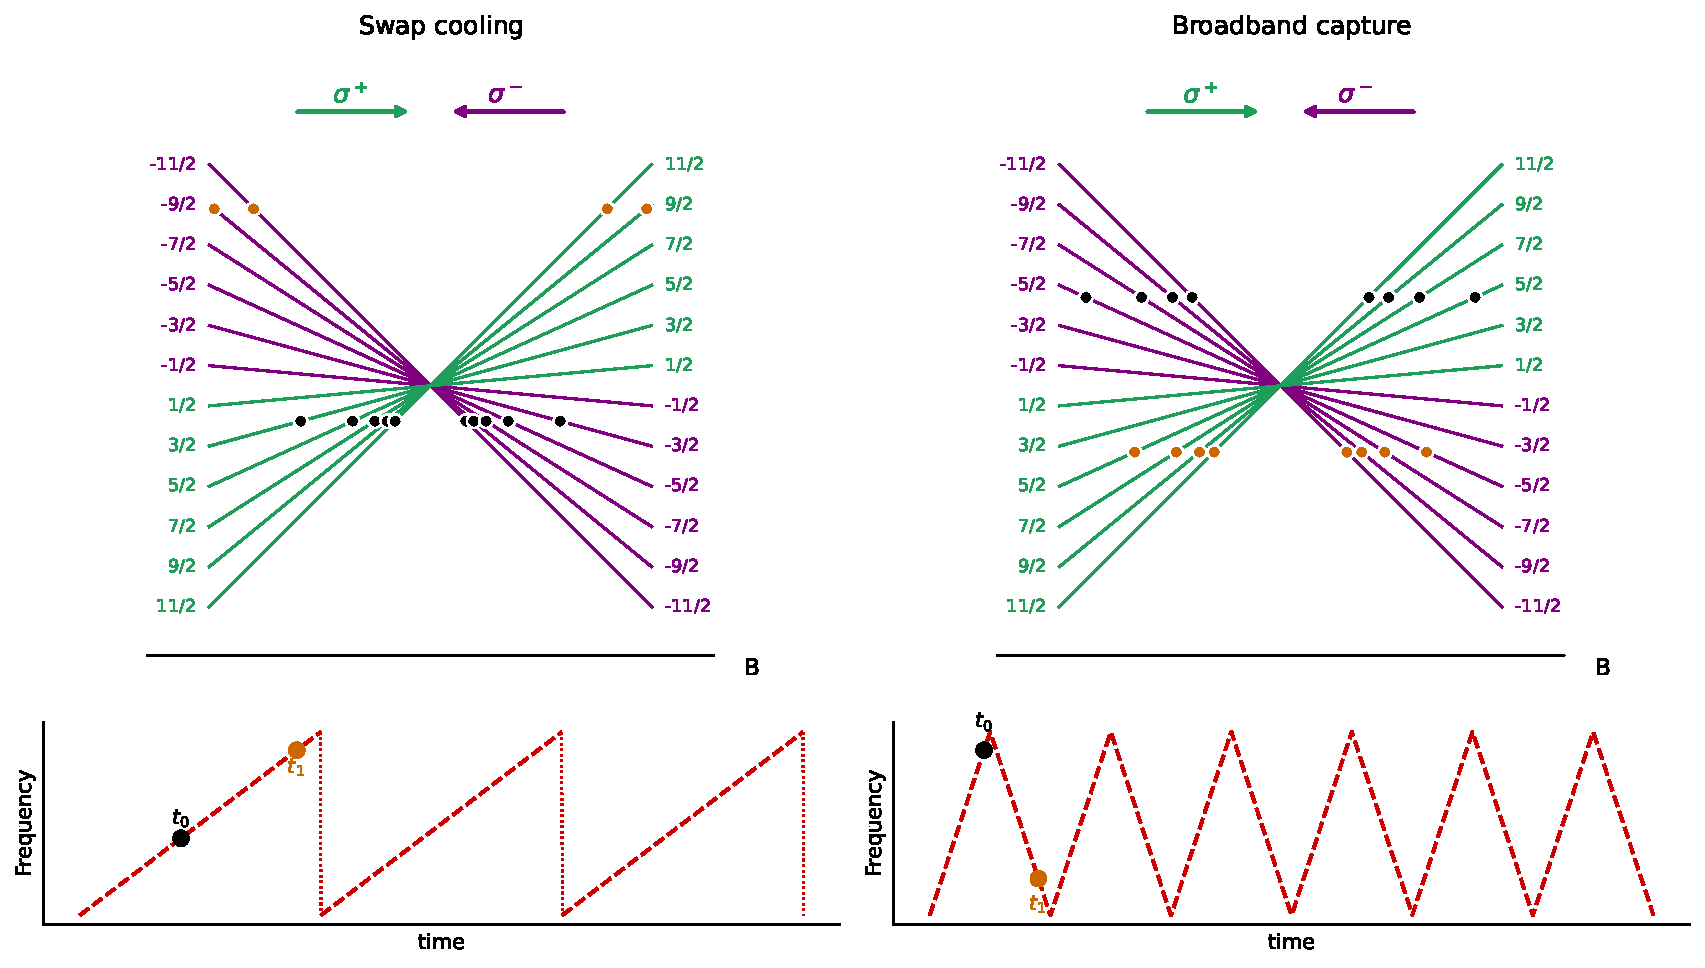
\includegraphics[width=1\linewidth]{Chapitres/Gas preparation and spin control/images/red_MOT_in_3_steps.pdf}
    \caption[Sequential stages of the $689~\text{nm}$ red MOT.]{Sequential stages of the $689~\text{nm}$ red MOT. From left to right : swap cooling and broadband capture (adapted from \cite{stellmerThesis}). The size of the cloud is decreasing with the cooling since the atoms are kicked in the opposite direction of the resonant laser of right polarization.}
    \label{fig:intro-red-mot-3-steps}
\end{figure}

\subsubsection{Optimization of narrowband MOT Parameters}

Cooling efficiency during the single-frequency stage depends on precise frequency, intensity, and timing parameters:
\begin{itemize}
    \item \textbf{Broadband modulation amplitude:} The initial sweep covers $\Delta f = 6~\text{MHz}$ on the atoms to capture the Doppler distribution from the blue MOT.
    
    \item \textbf{Intensity ramp and power broadening:} High intensities $I/I_{sat}=400 $ to 1600 provide a deep trap for initial capture, but causes power broadening ($\Gamma_{\text{eff}} = \Gamma \sqrt{1 + I/I_s}$), raising the achievable Doppler limit. For single-frequency cooling, intensity is adiabatically ramped down over $45~\text{ms}$ to reduce power broadening while maintaining sufficient force to support the cloud against gravity.
\end{itemize}
Atoms are adiabatically loaded into the ODT while decreasing the intensity of the
single-frequency $689~\text{nm}$ red MOT during a ramp lasting
approximately $45~\text{ms}$. From second-order perturbation theory, the light shift experienced by the energy levels yields
the optical dipole potential:
\begin{equation}
    U_{\text{dip}} = -\frac{\hbar|\Omega|^2}{4\bar{\Delta}}
\end{equation}
\cite{litvinov_these}, where $1/\bar{\Delta} = 1/(\omega_{\text{laser}} - \omega_{\text{atomic}}) - 1/(\omega_{\text{laser}} + \omega_{\text{atomic}})$ is the effective detuning factor, and $\Omega^2 = \frac{\Gamma^2}{2}\frac{I}{I_{\text{sat}}}$ is the Rabi frequency.

As seen from these expressions, the AC Stark shift induced by the dipole laser is state-dependent. As illustrated in Fig.~\ref{fig:intro-odt-loading}, the potential estimated in \cite{litvinov_these} is deeper for the ground state $^1S_0$ ($U_{\text{dip}}(^1S_0) \simeq -1.5~\text{MHz}$) than for the excited state $^3P_1$ ($U_{\text{dip}}(^3P_1) \simeq -1.2~\text{MHz}$) at the center of the trap, resulting in a differential blue-shift of the $^1S_0 \rightarrow {}^3P_1$ transition (black line)
compared to the frequency the atoms feel from the red MOT (red curve).

At the center, this shrinking gap is red-detuned from the MOT, enabling efficient cooling and confinement there. Away from
the center, the laser is blue-detuned from the trap which gives kinetic energy to the atoms accumulated at the edges of the 
ground state trap: these are the ones with the most kinetic energy we want to get rid off to reach ultracold temperatures.

\begin{figure}
    \centering
    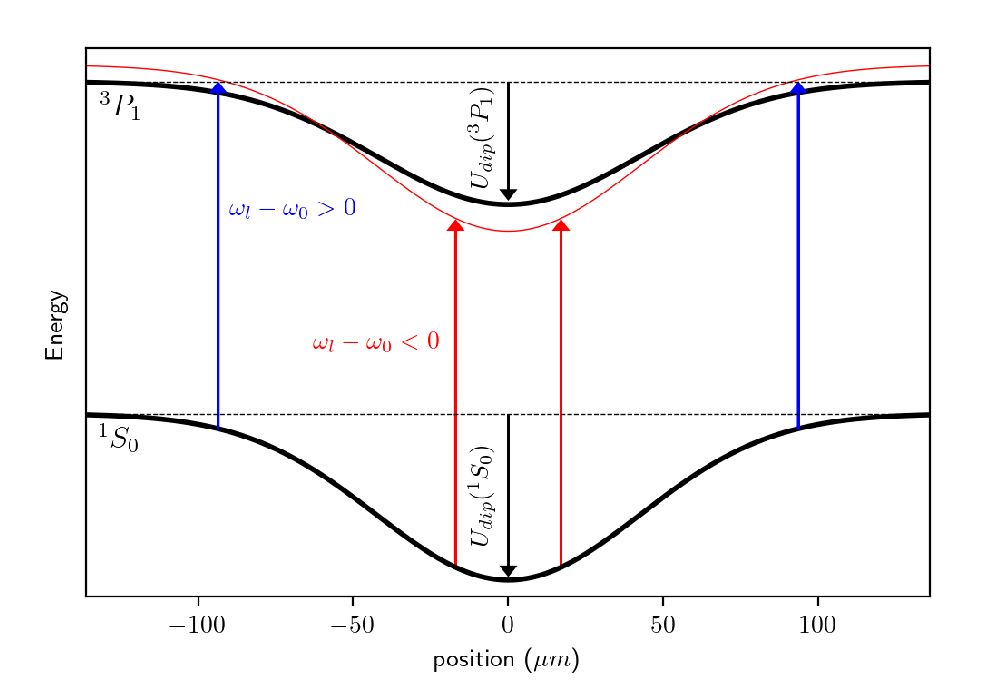
\includegraphics[width=0.9\linewidth]{Chapitres/Gas preparation and spin control/images/ODT_loading.pdf}
    \caption[Simulation extracted from \cite{litvinov_these}. Principle of localized $689~\text{nm}$ MOT loading inside the crossed optical dipole trap]{Simulation extracted from \cite{litvinov_these}. Principle of localized $689~\text{nm}$ MOT loading inside the crossed optical dipole trap due to the differential AC Stark shift between $^1S_0$ and $^3P_1$.}
    \label{fig:intro-odt-loading}
\end{figure}

Following loading, the $689~\text{nm}$ red MOT is switched off, and forced evaporative
cooling is performed purely by progressively lowering the ODT depth: the most energetic
atoms overcome the (now shallower) potential barrier and escape the trap, while the
remaining ones re-thermalize to lower temperatures via elastic collisions
(Fig.~\ref{fig:evap}). Incidentally, as the trap depth decreases, the differential AC
Stark shift also shrinks, so the local transition frequency at the trap center relaxes
back toward its unperturbed value -- though since the MOT laser is off at
this stage, this drift plays no role in the evaporation dynamics itself.

The results presented in the following two chapters were obtained with an atomic cloud located at the intersection of a horizontal beam, called the ``Reservoir'' (waist $w_0^H = 150~\mu\text{m}$), and a vertical beam, called the ``Dimple'' (waist $w_0^V = 80~\mu\text{m}$). The vertical beam axis is tilted at an angle of $\simeq 30^\circ$ relative to the vertical to facilitate the escape of the hottest atoms from the trap.

In Chapter 2, the horizontal arm is tilted by $\simeq 1^\circ$. For the photoassociation results in Chapter 3, this tilt was canceled: it enables to have bigger volumes to trap the atoms from the crossing of the two arms (see \ref{optimisation evap}).

Both $^1S_0$ and $^3P_1$ are shifted downward by the dipole trap potential, but $^1S_0$
experiences a larger shift due to its higher polarizability, so the energy difference between 
the two states is way more important at the center of the trap than on the edges. The atoms adressed by the 
red MOT laser at the center of the trapp are cooled with the red-detuned laser while the slighlty
blue-detuned laser is heating the atoms with the more kinetic energy -- located at the edges of the 
harmonic potential of the ODT -- in order to keep only the coldest atoms.


\begin{figure}
    \centering
    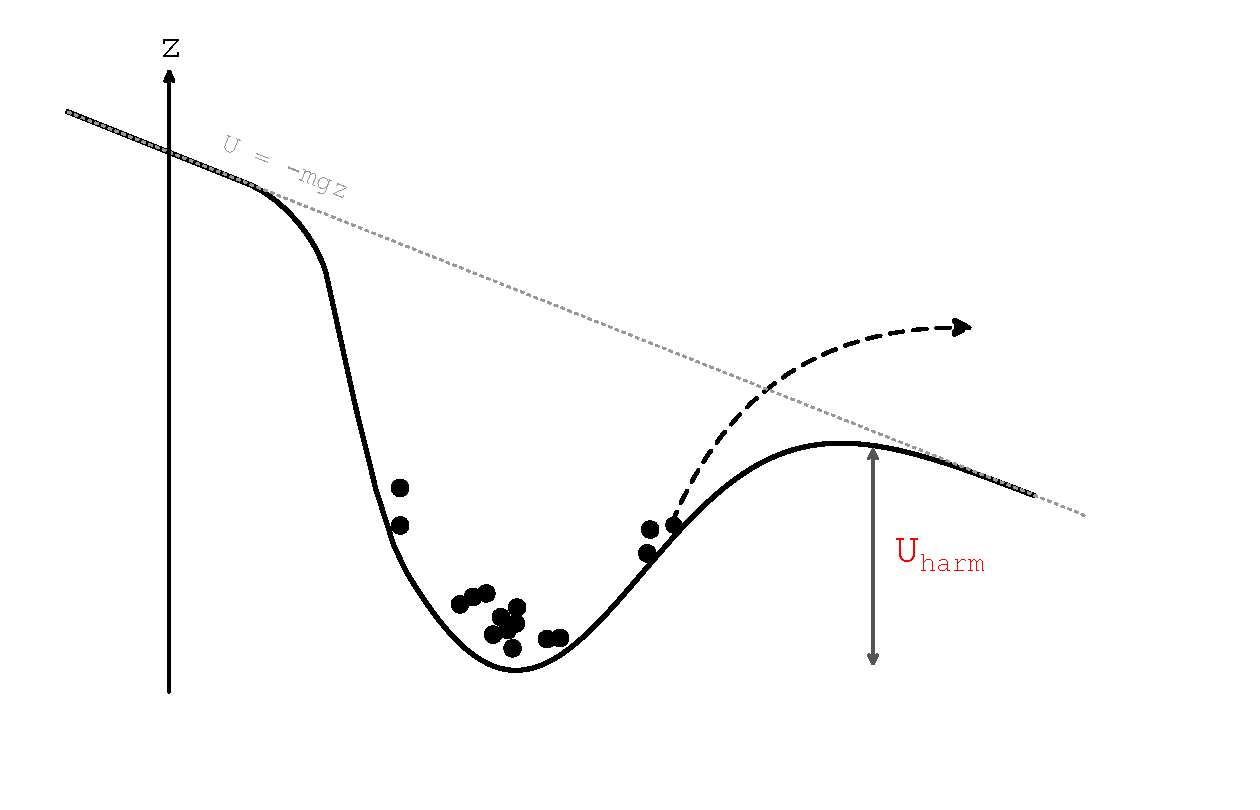
\includegraphics[width=0.7\linewidth]{Chapitres/Gas preparation and spin control/images/evaporative_cooling.pdf}
    \caption[Evaporative cooling mechanism in a crossed optical dipole trap]{Evaporative cooling mechanism in a crossed optical dipole trap, illustrating the escape of high-energy atoms and subsequent re-thermalization.}
    \label{fig:evap}
\end{figure}

\subsubsection{Optimization of the evaporation ramps}
\label{optimisation evap}
For a degenerate Fermi gas, the key parameter to optimize is the phase-space density (PSD), which scales as $\text{PSD} \propto N\bar{\omega}^3/T^3$, where $N$ is the atom number, $\bar{\omega}$ the geometrically averaged trap frequency, and $T$ the temperature. While both arms of the dipole trap influence these parameters, their main physical contributions differ:

\begin{itemize}
    \item \textbf{Tight vertical beam (``Dimple''):} Writing the atom number as $N = nV$ (where $n$ is the spatial density and $V$ the trap volume), the elastic collision rate scales as $\Gamma_{\text{el}} = n\sigma_{\text{el}}v_{\text{th}}$ with $\sigma_{el}$ the elastic collision cross section and $v_{th}$ the thermal speed of the atoms, enhancing collision rates for fast re-thermalization. This
    beam impacts mostly the temperature of the gas since it acts on the collision rate. The tightly focused waist of the dimple beam mainly dictates the local horizontal confinement, and contributes negligibly to the vertical confinement due to its near-vertical propagation axis~\cite{stellmer_production_2012}.

    \item \textbf{Broad horizontal beam (``Reservoir''):} Owing to its narrow vertical waist, the reservoir beam sets the effective trap depth $U$ against gravity-assisted atom loss, thereby controlling the evaporative truncation of the energy distribution and, in turn, the atom number~\cite{stellmer_production_2012}. Increasing the reservoir depth raises both $N$ (less truncation, more atoms retained) and $T$ (less evaporative cooling), and these two effects largely cancel out in the $N/T^3$ ratio: the reservoir therefore has a much weaker net effect on the PSD than the 
    dimple, whose action on $\bar\omega^3$ is not compensated by an opposite change in $N$. Therefore the reservoir compensates alone the gravity effect on the cloud. 

    \item \textbf{Ramp duration and adiabaticity:} The duration and adiabaticity of the evaporative ramps depend on the targeted state. Short evaporations are preferred when aiming solely for a large atom number at moderate temperatures when it is necessary to detect atom number fluctuations, such as for our experiments on photoassociation (see Chapt.3).
    Conversely, reaching deep quantum degeneracy requires a multi-stage ramp lasting approximately 7 seconds which was necessary for the results of Chapt.2.
\end{itemize}
For further details on loading atoms into the optical crossed dipole trap, the reader is referred to the thesis of A. Litvinov~\cite{litvinov_these}. An additional optical lattice, formed by a $1064~\text{nm}$ ALS laser, was initially implemented to enhance the phase-space density (PSD) of the atomic cloud prior to forced evaporative cooling. While this configuration was employed for the experiments presented in Chapter~2, it was subsequently discarded due to intensity fluctuations in the laser that induced significant heating.

\subsubsection{Optical setup}
The 1075 nm light from the IPG laser is split by a half-wave plate and polarizing beamsplitter into the two arms described above (Fig.~\ref{setup evap}). The horizontal arm forms the ``Reservoir'' beam: a pair of cylindrical lenses (f = -50 mm and f = -75 mm) shapes the elliptical beam into an anisotropic ellipse, with nominal waists of $w^h = 147~\mu$m (horizontal) and $w^v = 34~\mu$m (vertical) at the lens focal plane. However, the atoms sit $\simeq$ 3.3~mm beyond this focus rather than at the waist itself, so that the vertical waist they actually experience is somewhat
larger, $w^v \simeq 47~\mu$m, while the horizontal waist remains close to its nominal value at this distance. The second arm forms the ``Dimple'' beam, focused by a spherical lens (f = 300 mm) and crossing the reservoir arm at the position of the atoms, at $\simeq 30^\circ$ from vertical; astigmatism in this arm means its two transverse waists are not equidistant from the atoms either (measured at $\simeq$ 4.5~mm and $\simeq$ 7~mm, respectively).

\begin{figure}
    \centering
    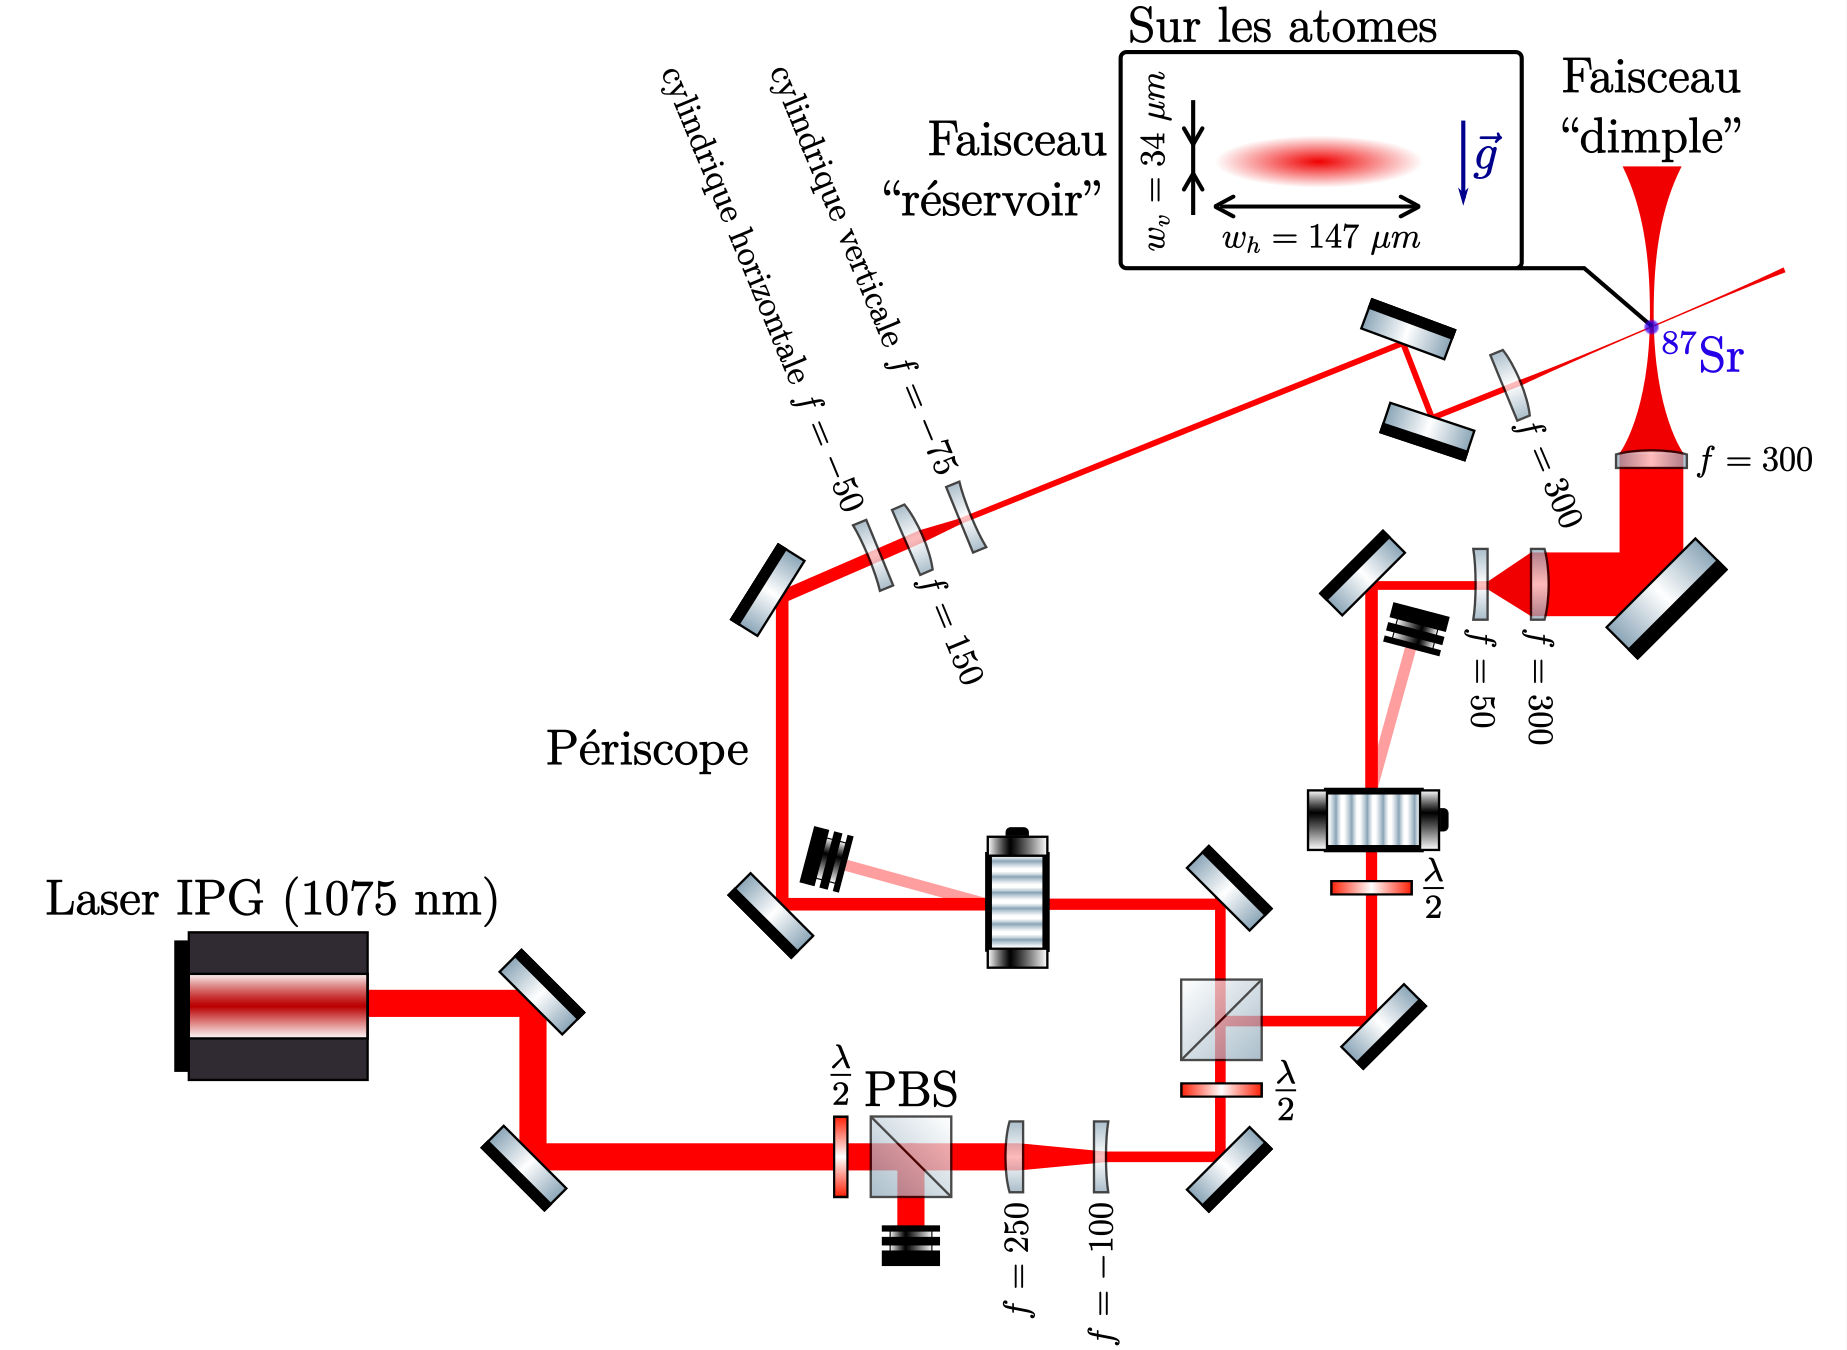
\includegraphics[width=1\linewidth]{Chapitres/Gas preparation and spin control/images/1.30_dipole_trap(1075)_setup.png}
    \caption{Optical setup of the 1075 nm crossed dipole trap laser system.}
    \label{setup evap}
\end{figure}

For the photoassociation measurements presented in Chapter 3, quantum degeneracy is not required, and a high atomic density is favored instead; these experiments are realized with 400 000 atoms of spread $\sigma \simeq 100~\mu$m at a few $\mu$K, as introduced above.

\section{Spin Selection}

\subsection{Optical Pumping}
Optical pumping is implemented prior to the final evaporation stages to prepare the atomic gas in a tailored mixture of nuclear spin states ($m_F$). Due to the $SU(N)$ symmetry of $^{87}\text{Sr}$, elastic $s$-wave collisions between identical fermions in the same $m_F$ state are forbidden by the Pauli exclusion principle. Therefore, at least two distinct spin components must be present to enable elastic collisions and ensure efficient re-thermalization during evaporative cooling. Furthermore, $SU(N)$ symmetry guarantees that elastic collisions conserve the nuclear spin state, preventing spin-exchange collisions during evaporation.

To perform state preparation, a bias magnetic field of $6.05 \pm 0.05~\text{G}$ is applied to lift the degeneracy of the $^3P_1, F = 11/2$ hyperfine sub-levels via the linear Zeeman effect. The cloud is illuminated by a $\sigma^-$-polarized optical pumping beam tuned to the $^1S_0 (F=9/2) \rightarrow {}^3P_1 (F=11/2)$ transition. Its frequency is defined as:
\begin{equation}
f_{11/2} = f_{\text{Radiant Dyes}} \pm f_{\text{Slave 1}}^{\text{RF}} + f_{11/2}^{\text{RF}}
\end{equation}
The sign goes depends on the wanted spin manipulation experiment (more details in chapter \ref{chap 3}).
The laser frequency is swept across 200~kHz around the targeted $^3P_1, F=11/2, m_F'$
sub-level -- to compensate for day-to-day energy shifts arising from experimental
fluctuations -- depleting the corresponding $^1S_0, F=9/2, m_F$ ground-state population
over about 5~ms at an intensity of $\simeq 70\,I_{\text{sat}}$. Spontaneous emission,
governed by the electric-dipole selection rule $\Delta m_F = 0, \pm 1$, then redistributes
the excited atoms into adjacent, lower-lying ground-state sub-levels, leading to a
progressive accumulation of population in the target spin states.

To prepare a specific mixture (e.g., a 2-spin mixture), unwanted spin populations are sequentially pumped out. One spin component, typically $m_F = -9/2$, is intentionally retained alongside the target mixture to maintain two-body elastic collisions for thermalization during evaporation. Once evaporative cooling is complete, this auxiliary component can be selectively removed using a short \textbf{'blast'} pulse. Under $\sigma^-$ excitation on the $F=9/2 \rightarrow F'=11/2$ transition, the $m_F = -9/2$ state couples exclusively to $m_F' = -11/2$. Because no $m_F = -11/2$ ground state exists, spontaneous emission from $m_F' = -11/2$ can only decay back to $m_F = -9/2$, forming a closed cycling transition. The resulting continuous photon scattering exerts a strong radiation pressure that expels the $m_F = -9/2$ population from the trap without disturbing the target single state or mixture. In practice, the blast pulse frequency is swept over a narrow range through resonance
(rather than held fixed) to make the removal insensitive to small drifts in laser
frequency or magnetic field calibration \cite{bataille_adiabatic_2020}.

\begin{figure}[H]
    \centering
    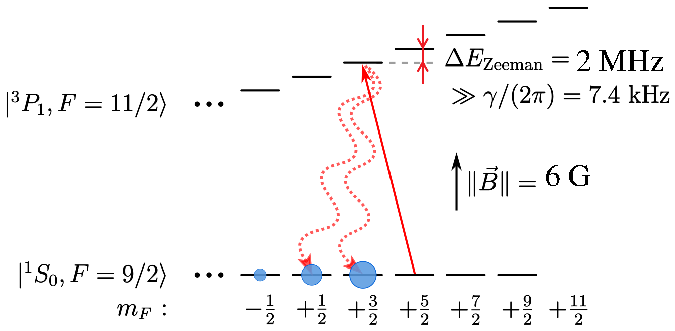
\includegraphics[width=1\linewidth]{Chapitres/Gas preparation and spin control/images/optical_pumping_bataille2020.pdf}
    \caption[Optical pumping scheme on the $^1S_0 (F=9/2) \rightarrow {}^3P_1 (F=11/2)$ transition]{Optical pumping scheme on the $^1S_0 (F=9/2) \rightarrow {}^3P_1 (F=11/2)$ transition used to prepare a specific nuclear spin mixture. The red laser is ramped through the target energy level of $^3P_1$: the atoms decay to neighbours states $m_F \pm 1$ of $^1S_0$}
    \label{fig:intro-optical-pumping}
\end{figure}

\section{Lasers for spin Manipulation}
We developed a method demonstrated in \cite{Bataille2020} for coherent control within the ground state manifold of zeeman sublevels. it relies on tensor shifts enacted by a laser operating near 689 nm, and will be described in detail in chapter 2. At a later stage, we performed photoassociation experiments in the vicinity of the intercombination manifold, see chapter 3. Both experiments actually rely on the same laser system, that I will present here.

\subsection{External Cavity Diode Laser (ECDL)}
\label{moglabs ecdl}
\subsubsection{Laser architecture}
The spin-selective method presented in the article \cite{Bataille2020} reveals the importance of inducing a Tensorial Light Shift (TLS) to be added to the Zeeman degeneracy lift.

For this purpose, an External Cavity Diode Laser (ECDL) from MOGlabs was chosen, whose architecture is shown in Fig.~\ref{fig:ecdl-laser}. A diode operating near $689~\text{nm}$
is first collimated by a collimation lens, before its frequency is roughly selected by an interference filter. The beam is then focused by a cat's-eye lens onto a partially reflective mirror placed at its focus -- represented by the dashed rectangular shape on the scheme. Together, this lens and mirror form a \textbf{cat's-eye retroreflector}: it compensates for any tilt of the wavefront introduced by the mirror, which would otherwise cause a loss of mode-matching with the light re-injected into the diode, and it closes the external cavity used to narrow and fine-tune the laser frequency. Most of the light reflected on the mirror sustains this resonant cavity, while the small transmitted fraction is collimated by an output lens and leaves the laser head through an optical isolator, with a linewidth below $100~\text{kHz}$.

\begin{figure}[H]
    \centering
    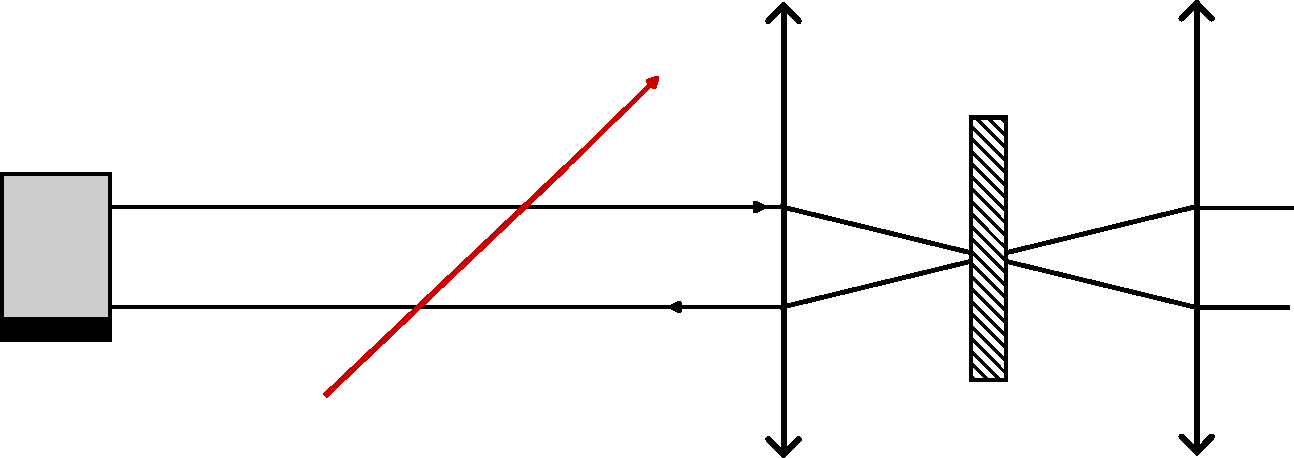
\includegraphics[width=0.9\linewidth]{Chapitres/Gas preparation and spin control/images/ecdl_cateye.pdf}
    \caption[MOGlabs External Cavity Diode Laser architecture used for spin manipulation]{MOGlabs External Cavity Diode Laser (ECDL) architecture used for spin manipulation. A diode lasing at 689~nm is first collimated by a lens, then its frequency is roughly selected by an interference filter marked in red. The beam is focused by a second lens onto a partially reflective mirror (hatched rectangle): together they form a cat's-eye retroreflector that closes the external cavity, feeding most of the light back for resonant frequency filtering while transmitting a small fraction onward. This output is collimated by a last lens and leaves the laser head through an optical isolator.}
    \label{fig:ecdl-laser}
\end{figure}

An internal PID controller robustly compensates for thermal and mechanical drifts of 
the cavity length as well as diode current fluctuations. The laser is subsequently beat-locked to a master optical reference adapted to the specific experimental requirements.

\subsubsection{Problems encountered on the MOGlabs ECDL}
For years, this ECDL exhibited a recurring instability that directly affected our experiments. We operate this laser far above threshold, at a fixed, high diode current chosen to maximize its output intensity on the external-cavity mode we lock to on a daily basis. As intracavity losses accumulated with time, however, the laser's entire mode spectrum -- the current-dependent map linking diode current to wavelength and output intensity -- drifted: at this same fixed operating current, the mode we needed was no longer the one giving maximum intensity, so the laser no longer delivered its usual output power on the intended wavelength. Rather than changing the operating current, we instead had to open the laser head and reduce the intracavity losses; lowering the laser's threshold in this way shifted the whole mode spectrum back, restoring the correspondence between our fixed operating current and maximum output intensity on the intended mode. This drift was eventually traced to two independent hardware issues, both responsible for a progressive loss of intracavity intensity:
\begin{itemize}
    \item the interference filter had developed damage at its center, degrading the transmission of the light. It was replaced with a new filter supplied by the manufacturer.
    \item one of the cavity's three piezoelectric actuators had failed. The full cat's-eye assembly was therefore replaced with an MGEF adapter featuring a wider-range frequency piezo.
\end{itemize}

Even after these repairs, a slow residual drift of the threshold persisted, now on a timescale of several days rather than hours. Gluing the cat's-eye assembly to the mount holding the diode and interference filter helped reduce this residual drift further, and keeping the laser switched off when not in use also limits it. If the stable mode eventually becomes inaccessible within the available diode current range, the threshold can still be lowered by gently adjusting the knobs of the mount holding the diode barrel. Because this realignment procedure slightly displaces the output beam, we added two optical fibers at the laser output: fiber coupling preserves the alignment to the rest of the spin-manipulation optical setup regardless of small beam-pointing changes.

\subsection{Optical bench for coherent Raman manipulations}

\subsubsection{Physical Concept}
The second chapter of this thesis focuses on spin manipulation within the $SU(10)$ manifold of $^{87}\text{Sr}$. This operation is realized via a two-photon Raman process driven by two laser beams red-detuned from the $^1S_0 \rightarrow {}^3P_1$ intercombination line.

Controlling the dimension of the effective Hilbert space from 1 to 10 requires independent addressing of individual spin states. The two-photon Rabi frequency $\Omega$ coupling two ground-state sub-levels $\ket{g, m_F}$ and $\ket{g, m_F'}$ through intermediate excited states $\ket{e}$ takes the form:
\begin{equation}
\hbar \Omega = \sum_{e} \frac{\bra{g, m_F'} \vec{d} \cdot \vec{E}_2^* \ket{e} \bra{e} \vec{d} \cdot \vec{E}_1 \ket{g, m_F}}{\Delta_e}
\end{equation}
where $\vec{d}$ is the dipole operator, $\vec{E}_1, \vec{E}_2$ are the electric field amplitudes, and $\Delta_e$ is the single-photon detuning relative to the intermediate state $\ket{e}$.

By applying the TLS, the energy difference between two consecutive spin projections $m_F$ and $m_F+1$ becomes non-linear:
\begin{equation}
\Delta E_{m_F}^{m_F+1} = q(2 m_F + 1) + \beta
\end{equation}
where $q$ parameterizes the quadratic (tensor) light shift and $\beta$ represents the linear Zeeman contribution. This explicit dependence on $m_F$ lifts the energy degeneracy between adjacent transitions, allowing spectral isolation and individual control of any given $m_F \leftrightarrow m_F+1$ pair.

\begin{figure}[H]
\centering
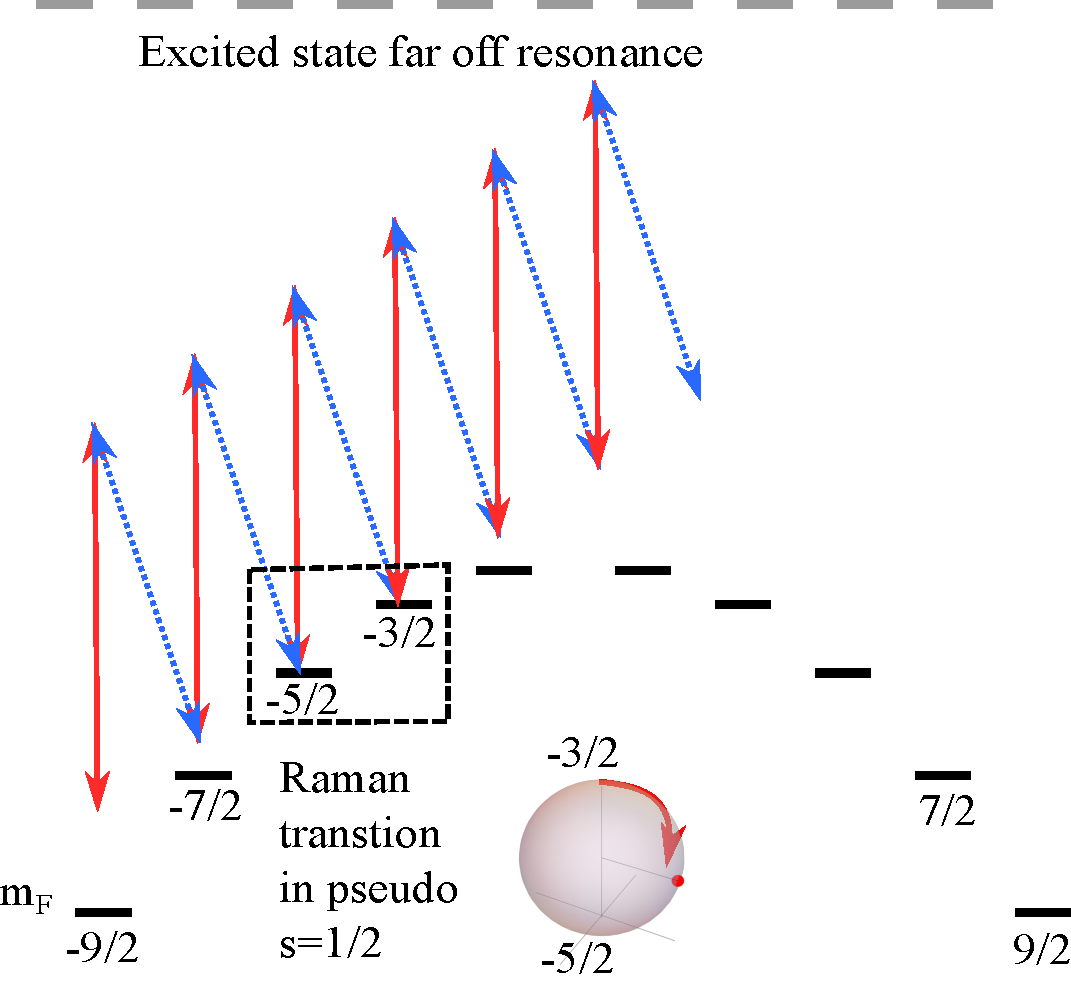
\includegraphics[width=0.9\linewidth]{Chapitres/Gas preparation and spin control/images/TLS_et_raman.pdf}
\caption[Spin manipulation scheme extracted from \cite{bataille_realisation_nodate}]{Spin manipulation scheme of \cite{bataille_realisation_nodate}. The isolation of spin states is allowed by the tensorial shift of the ground states that makes neighbours $m_F$ states isolated from the other resonances.}
\label{fig:tls-raman-scheme}
\end{figure}

For more details this process is discussed in the second chapter of this thesis and also in the article of the group \cite{Bataille2020}.

\subsubsection{Experimental Setup of the Raman process}
The two-photon process is driven by two distinct beams: a first beam derived from the ``AOM TLS'' laser (shown in red in Fig.~\ref{fig:raman-transitions}) generates the TLS and supplies the first photon. A second beam, frequency-shifted by the ``AOM Raman'' (shown in blue), completes the Raman transition.

The TLS beam polarization is set parallel to the magnetic field ($\pi$ transitions), producing a purely scalar/tensor light shift with no vector component. The Raman beam polarization is linear and orthogonal to the magnetic field, so that its decomposition onto $\sigma^+$ and $\sigma^-$ components drives the required $\Delta m_F = \pm 1$ legs of the two-photon transition -- one photon absorbed from the $\pi$-polarized TLS beam, one photon emitted into the $\sigma^{\mp}$ component of the Raman beam.
Both beams are copropagating in the same polarization maintening fiber with perpendicular polarizations preserving any interferencies that could affect the process.
This configuration selectively couples a single pair of states—for instance,\linebreak $\ket{^1S_0, F=9/2, m_F=-7/2} \leftrightarrow \ket{^1S_0, F=9/2, m_F=-5/2}$ —while remaining far off-resonance for all other $m_F$ states. The two-photon Raman coupling strength scales as $\Omega_R \propto \sqrt{I_{D} I_R}$, while the spacing between adjacent Raman resonances scales as $2q/h \propto I_{D}$. Spectral isolation of a single $m_F \leftrightarrow m_F'$ pair therefore requires $I_R \ll I_{D}$, so that neighbouring resonances remain spectrally resolved; in practice we use $I_R/I_{D} \lesssim 10^{-4}$ \cite{bataille_realisation_nodate}.

The complete optical path for this two-photon process, together with the filtering cavity described in Sec.~\ref{FP cavity}, is shown in Fig.~\ref{fig:raman-transitions}.

\begin{figure}[H]
    \centering
    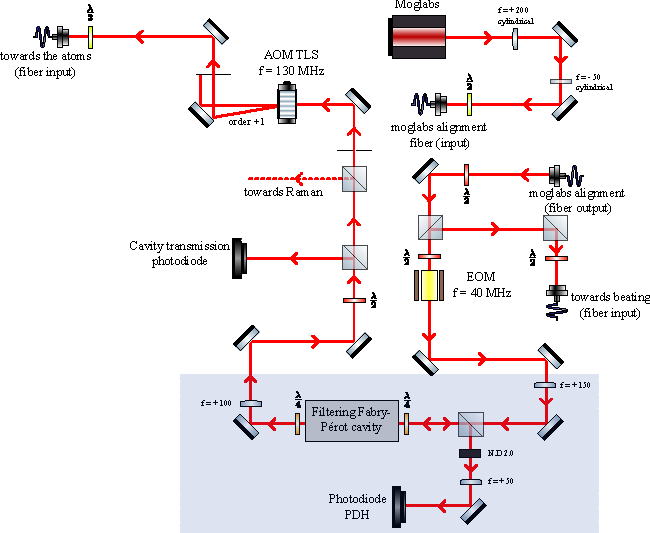
\includegraphics[width=1\linewidth]{Chapitres/Gas preparation and spin control/images/moglab.pdf}
    \caption{Complete optical setup including the Fabry-Pérot cavity and PDH stabilization loop.}
    \label{fig:raman-transitions}
\end{figure}

To reduce amplified spontaneous emission (ASE) from the laser source -- and thereby minimize stray light and photon-recoil heating during spin manipulation -- the optical chain incorporates a custom-built, PDH-stabilized confocal Fabry-Pérot cavity, detailed in Sec.~\ref{FP cavity}. The effect of the ASE has been observed by the heating of the gas while the laser was 
hundred's of MHz off resonance of transitions where we expect really low spontaneous emission. This cavity was originally built with these Raman TLS experiments in mind; however, by the time its construction was completed the corresponding measurements had already been carried out, and the experimental effort had moved on to the photoassociation spectroscopy presented in Chapter 3 -- for which the cavity turned out to be essential, given the higher sensitivity of these measurements to stray light. It is intended to be used again for future extensions of the Chapter 2 spin-manipulation experiments.

\subsection{Optical bench for photoassociation experiments}
Chapter 3 investigates photoassociation spectroscopy below the intercombination line. For these measurements, the full power of the laser is sent through the ``AOM lattice 689'' since the other AOM is not useful anymore, and the filtering cavity introduced above (Sec.~\ref{FP cavity}) is used for all datasets presented in that chapter.

\subsection{Fabry-Pérot cavity and PDH Locking system}
\label{FP cavity}
\subsubsection{Cavity design and assembly}

A primary objective of the cavity injection scheme in our optical setup is to maximize overall transmission for spin manipulation. To achieve this, 
we constructed a confocal cavity configuration ($d_0 = R_C$, where $d_0$ is the mirror separation and $R_C$ is their radius of curvature), ensuring 
that all odd transverse modes are degenerate and resonate at the same frequency. If these modes were non-degenerate, off-resonance spatial components 
would be reflected at the input mirror, thereby reducing the total cavity transmission efficiency.

In addition to the confocal geometry, longitudinal mode resonance requires that the cavity length $d_0$ satisfies the condition:
\begin{equation}
d_0 = n \frac{\lambda}{2}
\label{eq:cavity_resonance}
\end{equation}
where $n$ is an integer and $\lambda$ is the wavelength of the injection laser.

To fulfill these requirements, we selected curved mirrors with a diameter of $D = 4.5 \pm 0.15~\text{mm}$ and a radius of curvature matching $d_0$. The manufacturer specified a nominal mirror transmission of $T_{\text{mirror}} = 1.28\%$, though the effective system performance can be influenced by mechanical mounting constraints.

Proper cavity operation requires the mirrors to be aligned precisely parallel to each other and perpendicular to the optical propagation axis. In our initial implementation (Fig.~\ref{miroirs cav before} top), the mirrors were permanently glued into place. However, this approach introduced major technical issues over time: excess glue migrated onto the optical surfaces, degrading overall transmission, while alignment errors during gluing introduced an uncorrected angular tilt relative to the beam axis.

\begin{figure}[H]
    \centering
    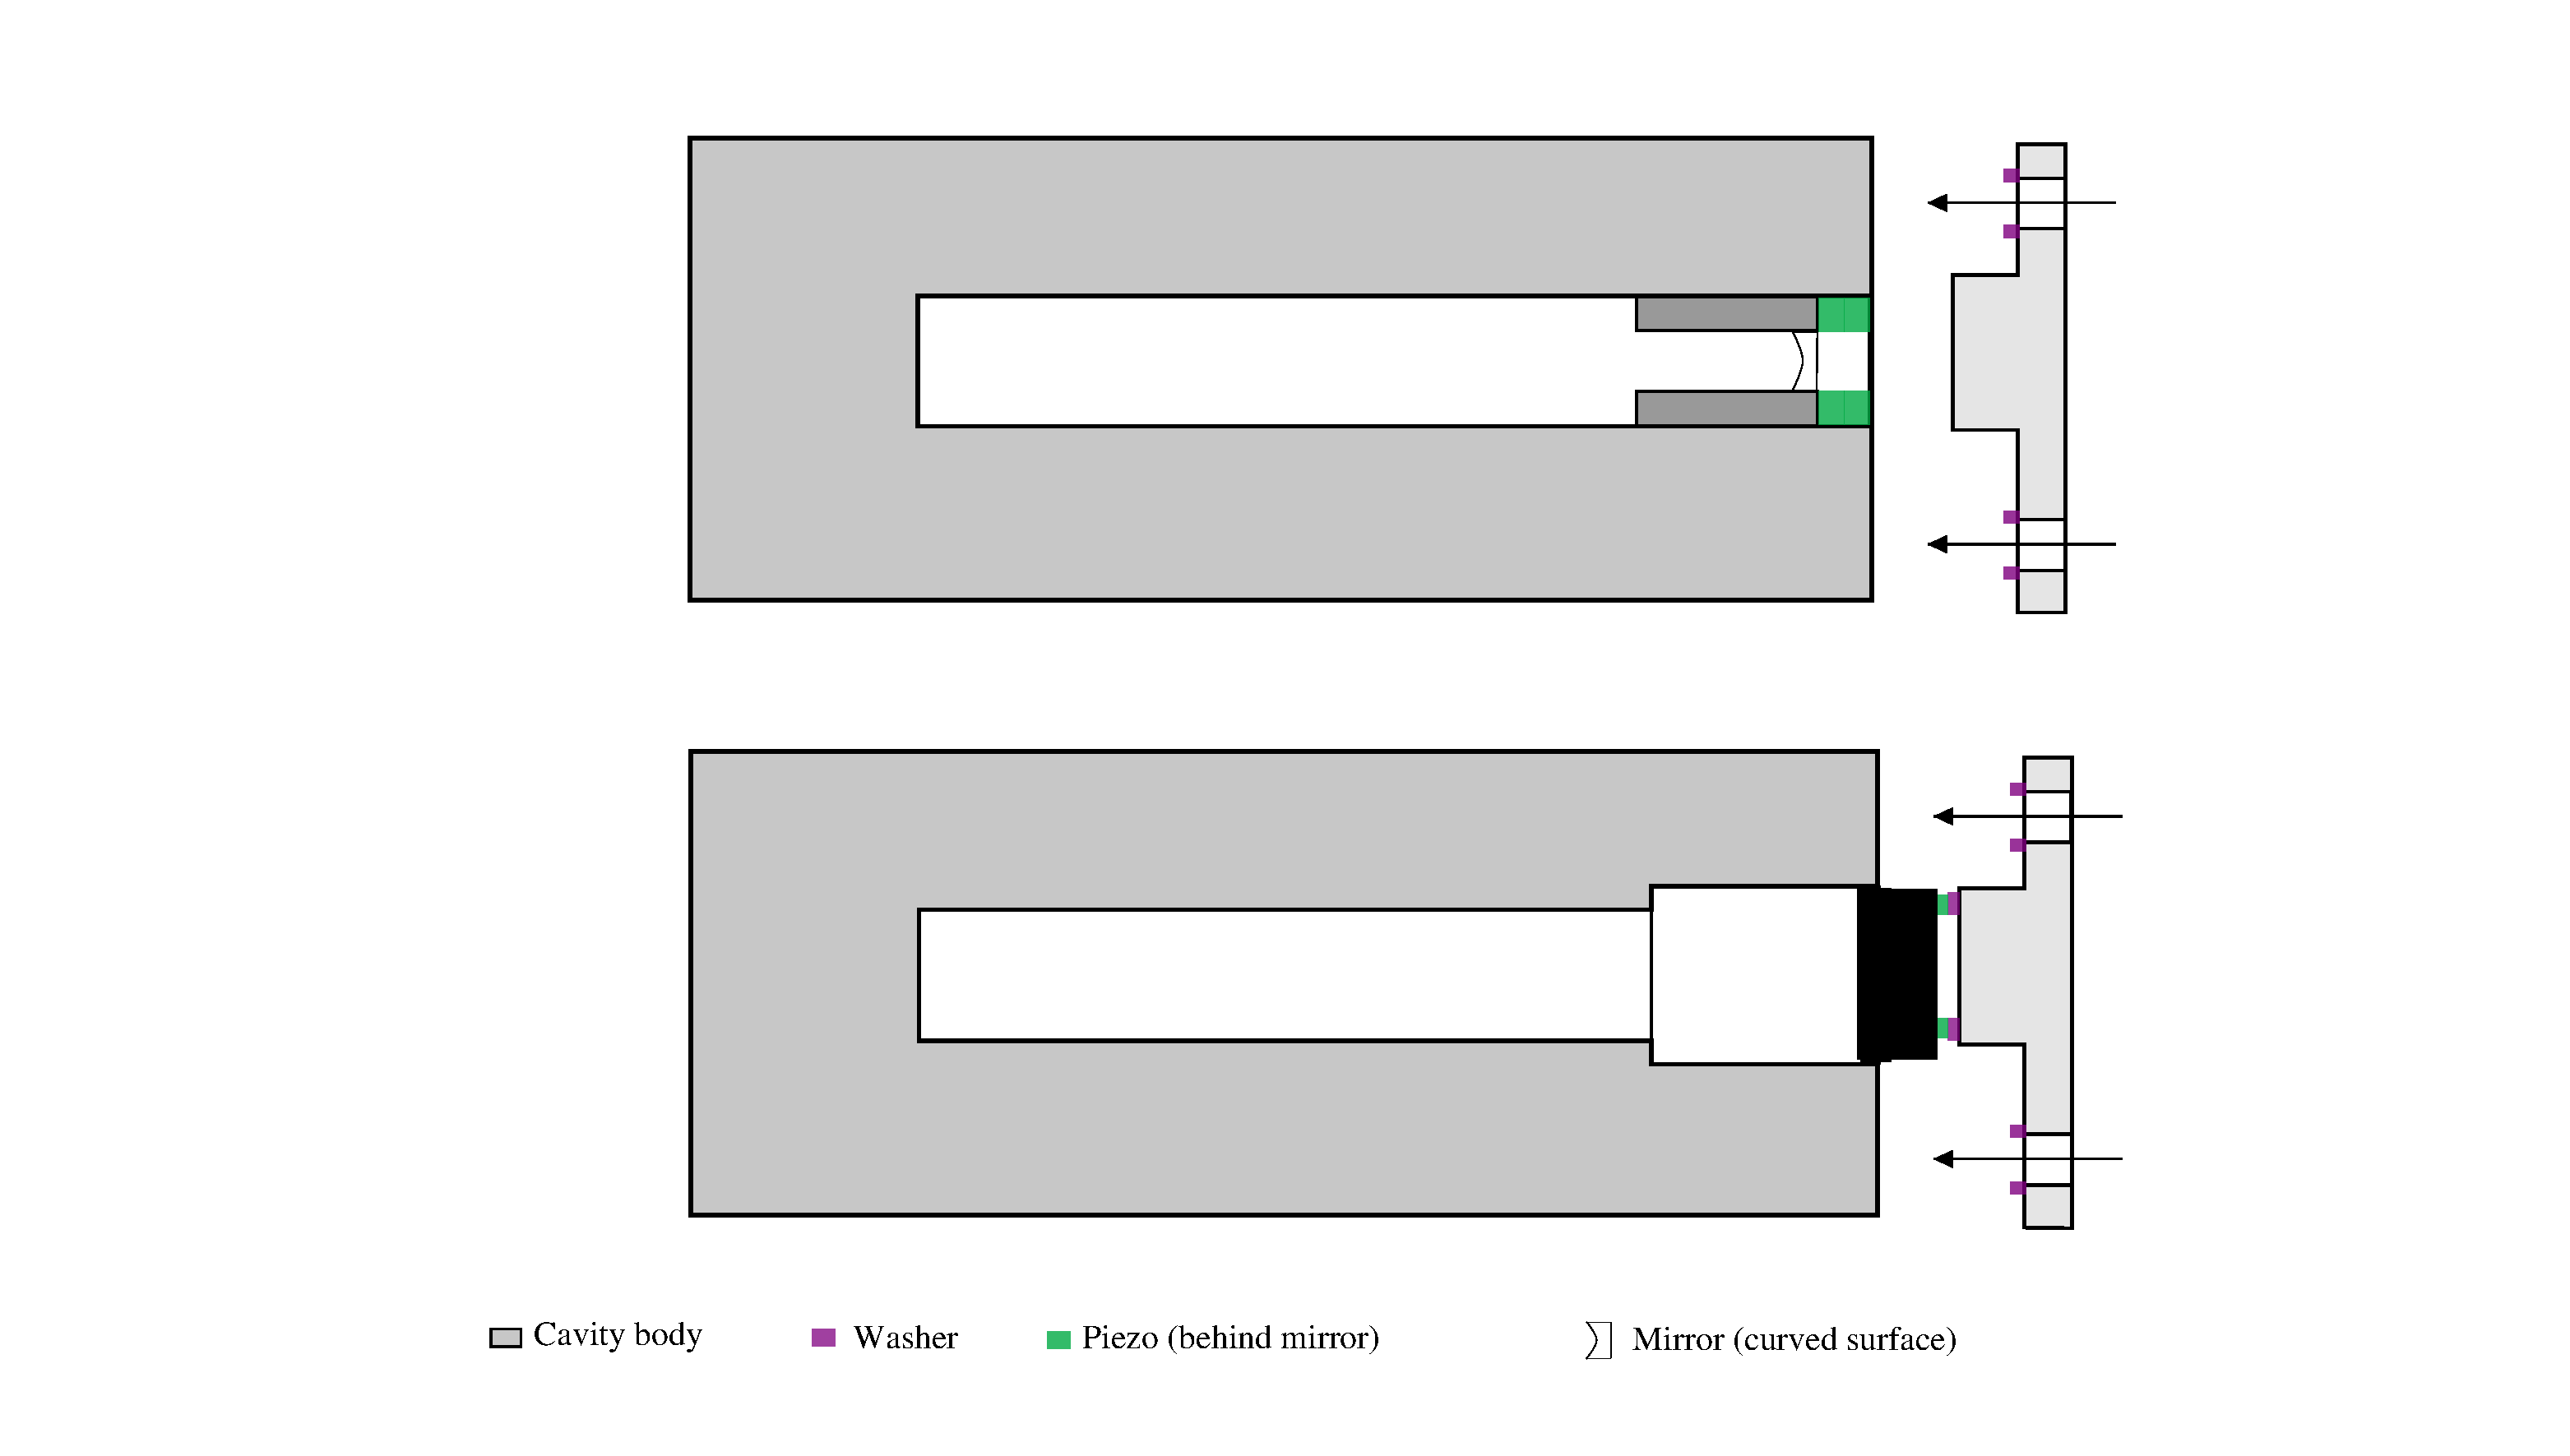
\includegraphics[width=1\linewidth]{Chapitres/Gas preparation and spin control/images/cavity_mount.pdf}
    \caption[Fabry-Pérot comparison of cavity construction method]{Top : Initial fixed cavity assembly using glued mirrors, lacking mechanical alignment degrees of freedom. Bottom : Upgraded and final cavity mount featuring three adjustment screws and compliant washers for precise angular and longitudinal alignment}
    \label{miroirs cav before}
\end{figure}

Because the original design provided no mechanical degrees of freedom to correct these misalignments, we redesigned the mounting mechanism. The updated cavity assembly is presented in Fig.~\ref{miroirs cav before} bottom. In this configuration, three adjustment knobs on a circular outer mount apply controlled pressure against the central cylindrical spacer housing the mirrors, with intermediate washers providing mechanical compliance. This allows for precise tilt control and fine adjustment of the mirror separation.

An additional parameter that has been adjusted during the construction is the mass of the 
mirrors: a first generation of the cavity has been constructed with heavier mirrors than 
actual ones, which presented mechanical resonance in the acoustic frequency range. The lock
of the cavity was not robust. Then this new generation is made of smaller and light mirrors
which pushes these resonances to higher frequency range we do not bother.

Once locked to the injection laser, the optimized cavity achieves a total power
transmission efficiency of $T = 0.63$. This limited efficiency likely results from
residual mechanical imperfections inherited from the original glued assembly: a slight
angular mis-gluing of a mirror could tilt the cavity axis and cause part of the beam to
clip inside the cavity, while leftover glue or dirt on the mirror surfaces could add
further scattering losses. Despite this imperfect transmission, the cavity's spectral
properties remain well characterized. The Free Spectral Range (FSR) of the cavity is
given by:
\begin{equation}
\text{FSR} = \frac{c}{2 d_0} = 3~\text{GHz}
\end{equation}
with a measured finesse of:
\begin{equation}
\mathcal{F} = \frac{\text{FSR}}{\delta \nu} = 310 \pm 15
\end{equation}
where $\delta \nu$ represents the full width at half maximum (FWHM) of the transmitted
resonance peak measured on a photodiode for the odd transverse modes.


\subsubsection{Pound-Drever-Hall locking system and PID controller analysis}

The cavity is frequency-locked to the laser using the Pound-Drever-Hall (PDH) technique, as detailed by Black~\cite{black_Gas_preparation_and_spin_control_2001} and schematized in Fig.~\ref{fig:pid}. The scheme utilizes an Electro-Optic Modulator (EOM) to generate sidebands at frequencies $f_0 \pm f_M$ around the optical carrier $f_0$, with a modulation frequency of $f_M = 40.48~\text{MHz}$. The modulated electric field incident on the cavity is expressed as:
\begin{equation}
E_{\text{inc}}^{\text{mod}} \approx E_0 \left[ J_0(\beta) e^{i 2\pi f_0 t} + J_1(\beta) e^{i 2\pi (f_0 + f_M) t} - J_1(\beta) e^{i 2\pi (f_0 - f_M) t} \right]
\end{equation}
where $J_0(\beta)$ and $J_1(\beta)$ are the zeroth- and first-order Bessel functions of the first kind, and $\beta$ is the modulation index.

\begin{figure}[H]
    \centering
    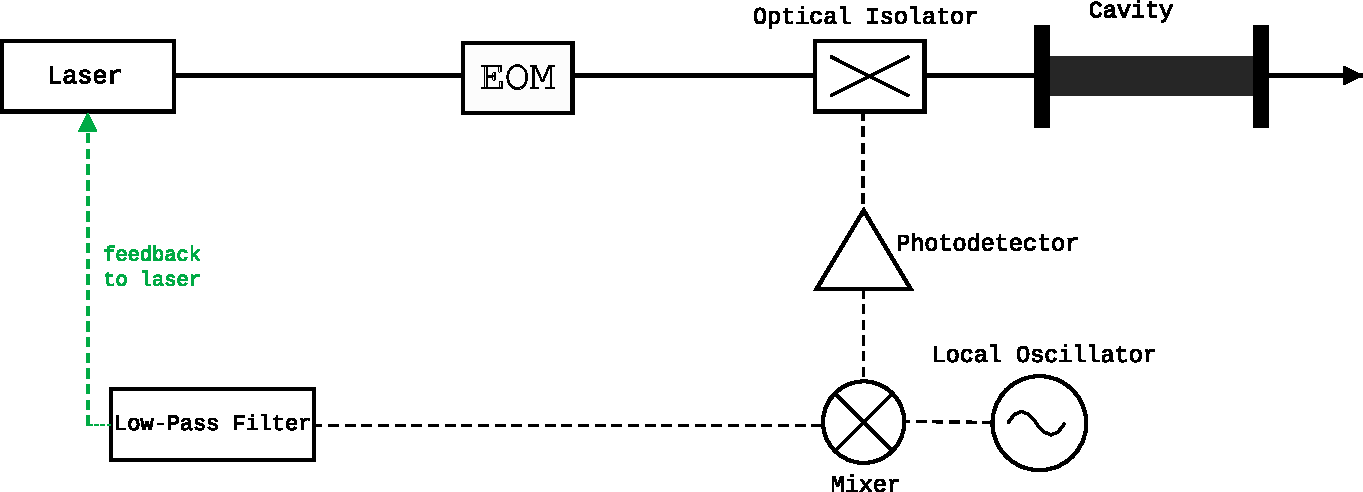
\includegraphics[width=1\linewidth]{Chapitres/Gas preparation and spin control/images/PID_black.pdf}
    \caption[Schematic of the Pound-Drever-Hall locking system]{Schematic of the Pound-Drever-Hall locking system, extracted and adapted from \cite{black_Gas_preparation_and_spin_control_2001}. The laser is firstly passing through an EOM that is modulating the eletric field at frequency $f_M$, creating two sidebands at frequency $f_{laser}\pm f_M$. The carrier at $f_{laser}$ and the sidebands are passing through the filtering Fabry-Pérot cavity wich is reflecting the light going back to the entrance of the cavity. 
    A beamsplitter serving as an optical isolator is reflecting the light to a photodiode. Then this signal is mixed with a local oscillator to extract an error signal to which a low-pass filter is combined to keep only the signal for the locking.}
    \label{fig:pid}
\end{figure}

The carrier enters the cavity and acquires a steep, frequency-dependent phase shift near resonance, whereas the sidebands are promptly reflected from the input mirror. The interference between the reflected carrier and the sidebands is detected on a fast photodiode, demodulated at $f_M$, and low-pass filtered to extract the dispersive error signal (Fig.~\ref{fig:pdh-error-signal}). The sharp linear slope around resonance provides a robust error signal highly sensitive to the sign of the frequency excursion.
From this graph, one measures a signal-to-noise ratio of SNR = 187. Interestingly, the sideband resonance features were not distinctly visible on the scanning error signal, even when driving the EOM with a high modulation depth to maximize the $J_1/J_0$ ratio.

 \begin{figure}[H]
    \centering
    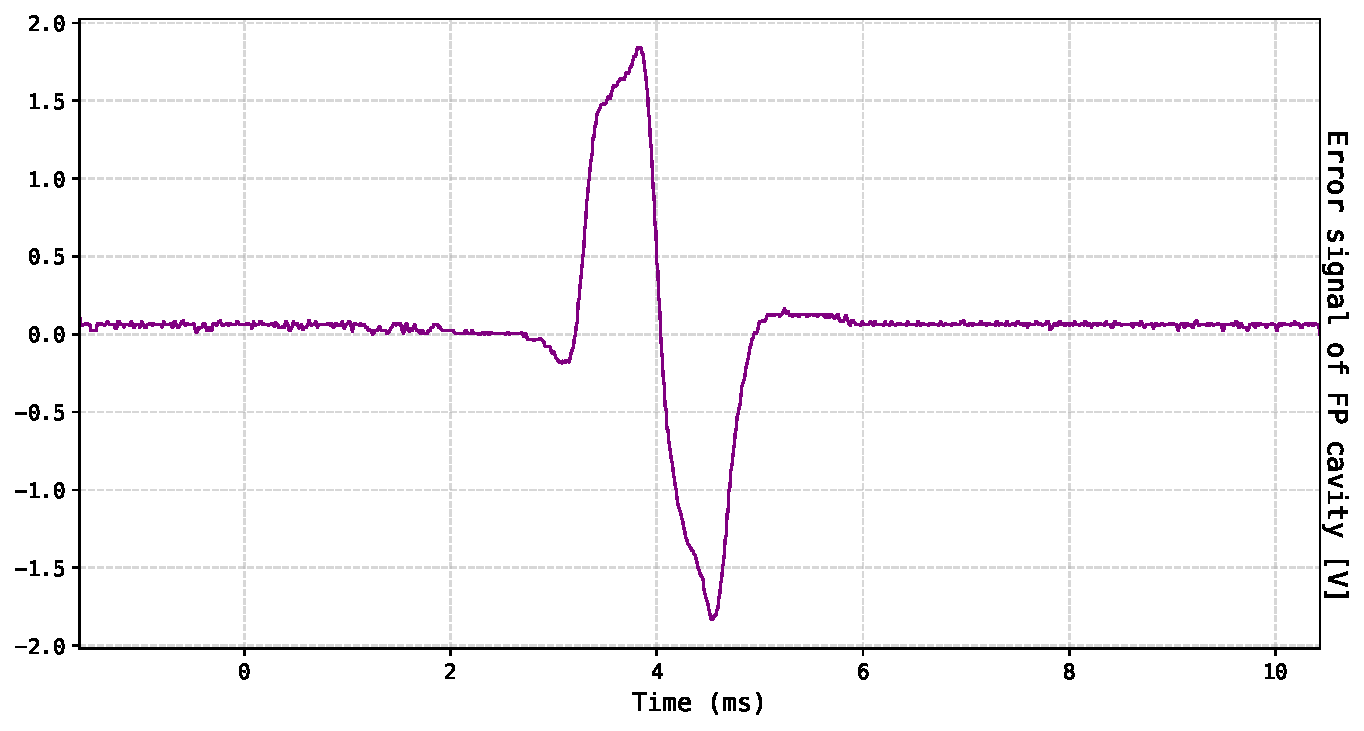
\includegraphics[width=1\linewidth]{Chapitres/Gas preparation and spin control/images/error_signal_FP.pdf}
    \caption[Pound-Drever-Hall error signal of the homemade Fabry-Pérot cavity]{Pound-Drever-Hall (PDH) error signal obtained by scanning the cavity length across resonance, enabling the lock cavity for the filtering of MOGlabs laser.}
    \label{fig:pdh-error-signal}
\end{figure}

Digital feedback control and noise analysis were implemented primarily using a Red Pitaya
STEMlab board, driving a home-made PID controller with separate proportional and
integral stages (Fig.~\ref{lock PID}), which we found sufficient for our setup. The PID
parameters were optimized by injecting a broadband electronic noise signal into the
cavity piezo driver and measuring the closed-loop transfer function. As seen in the
frequency response plot (Fig.~\ref{fig:analyse_bruit}), operating the system with
specific gain values excites mechanical resonances at low frequencies, with at 3~kHz 
the electronical bump that has similar amplitude for every gain but that is pushed to 
higher frequencies while the gain increases. 
Consequently, the final feedback loop acting on the cavity incorporates a
low-pass filter with a cut-off frequency of $f_c = 40~\text{kHz}$, a proportional gain
strictly bounded between $1 < K_p < 10$, and an integral gain configured between
$0 < K_i < 8~\text{s}^{-1}$.

\begin{figure}[H]
    \centering
    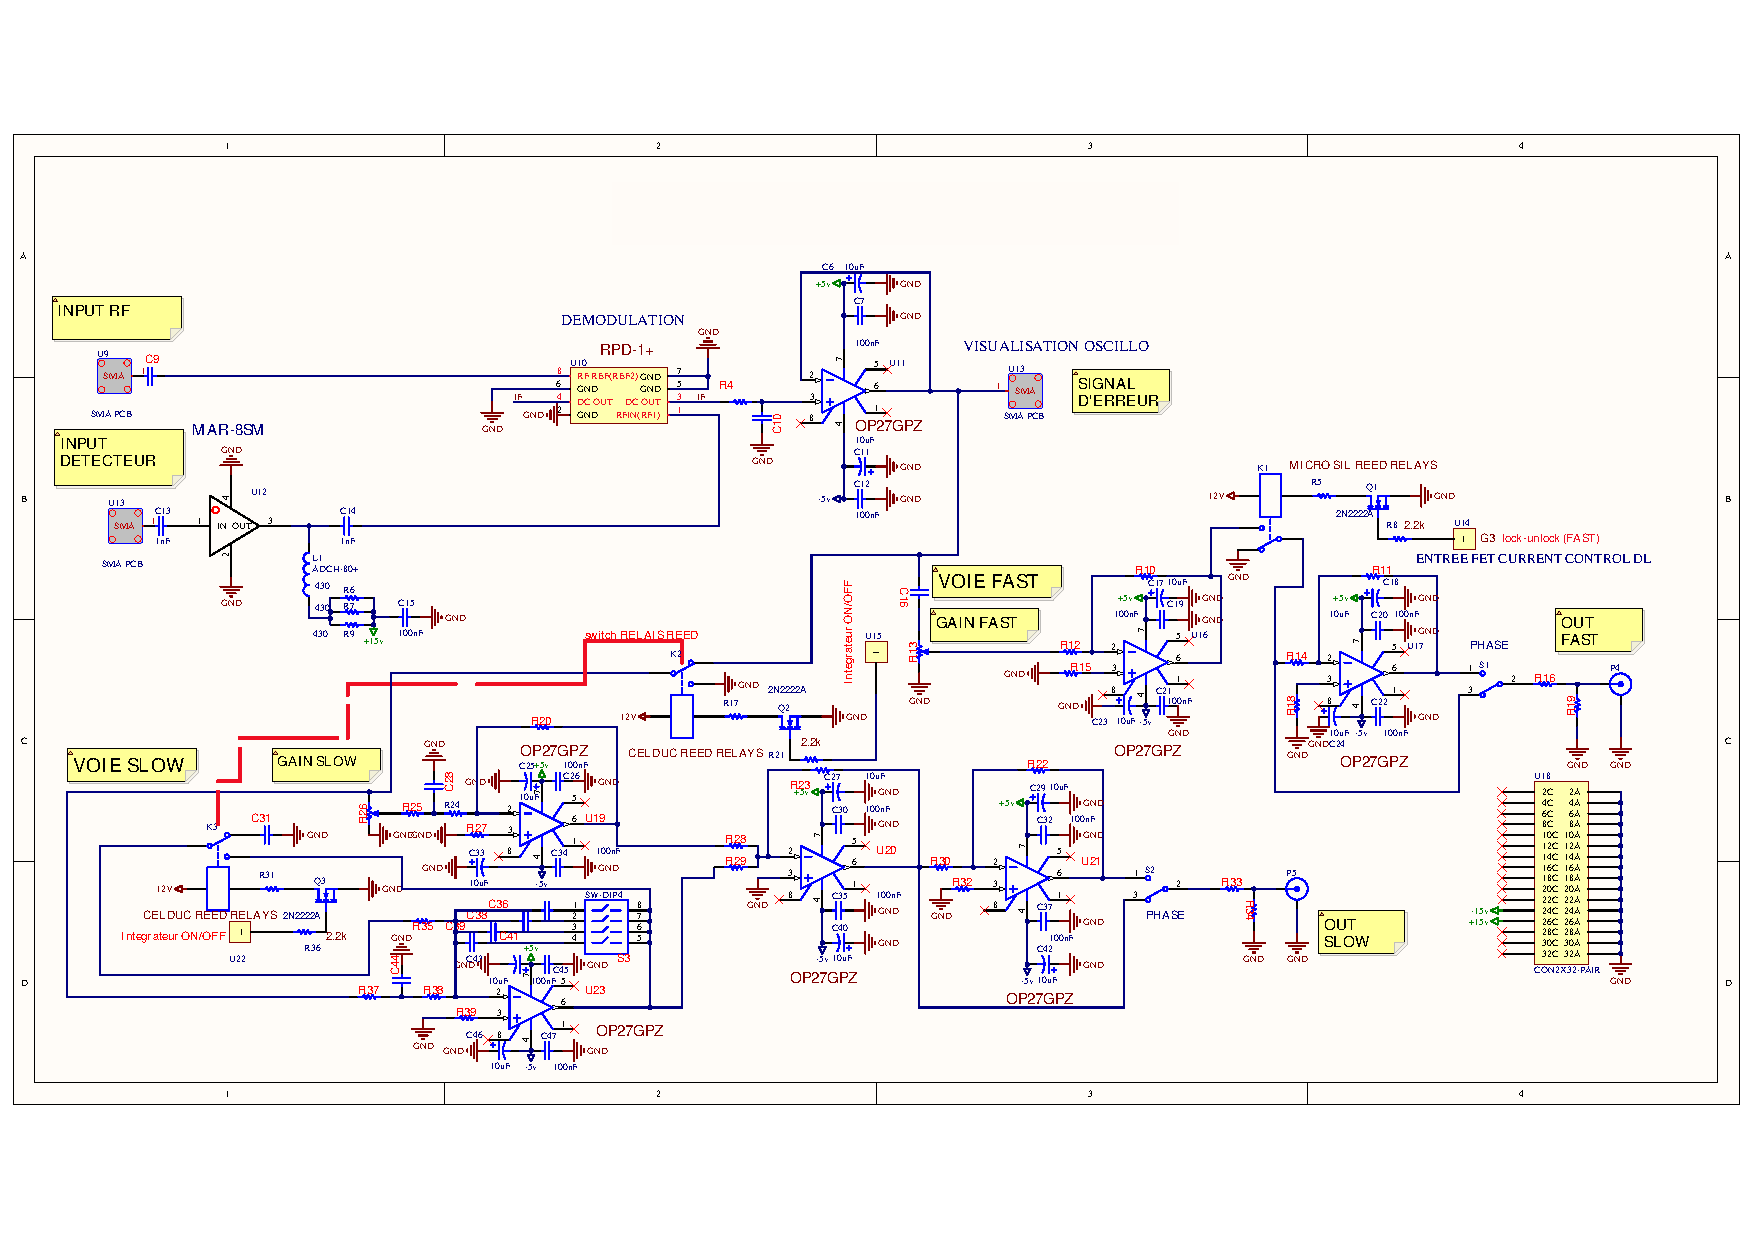
\includegraphics[width=1\linewidth]{Chapitres/Gas preparation and spin control/images/Carte_lock_laser_PDH_sr1sr2.pdf}
    \caption[Homemade PID scheme]{Homemade PID scheme constructed by the Fabrice Wiotte from electronic workshop of LPL. It is composed of separate proportional and integral stages, which we considered sufficient for our setup.}
    \label{lock PID}
\end{figure}

\begin{figure}[H]
    \centering
    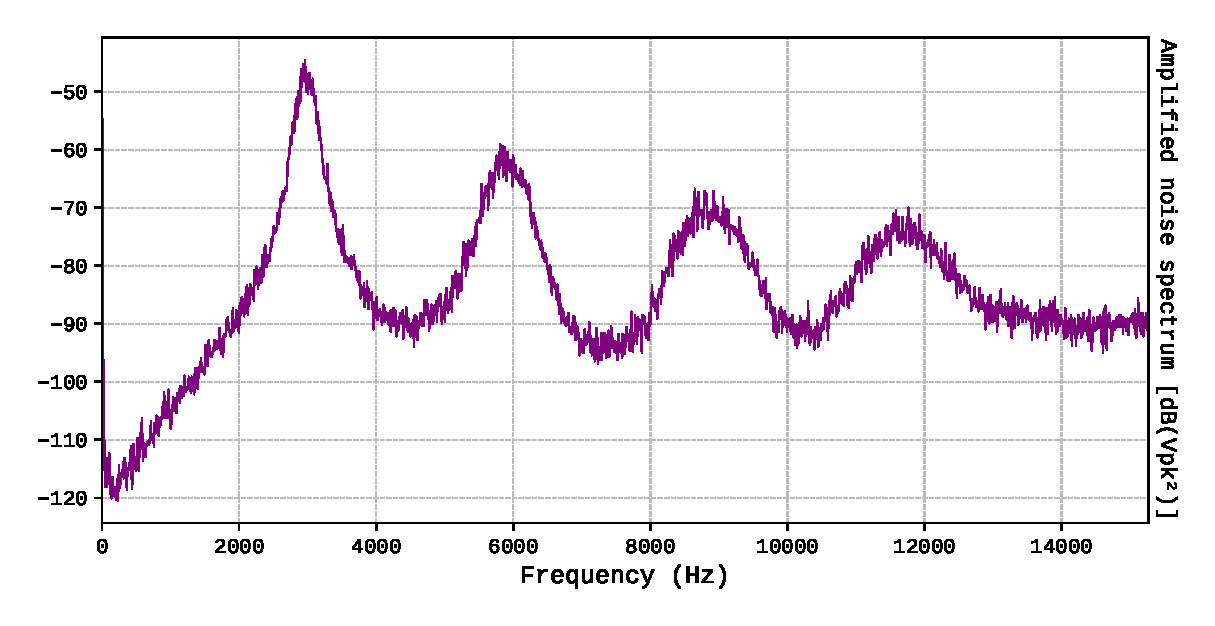
\includegraphics[width=1\linewidth]{Chapitres/Gas preparation and spin control/images/noise_spectrum.pdf}
    \caption[Closed-loop noise analysis of the Fabry-Pérot cavity]{Closed-loop noise analysis and mechanical resonance identification using the Red Pitaya with a gain that is amplifying parasitic noise, such as the mechanical resonance of the piezo at $f = 35~$kHz.}
    \label{fig:analyse_bruit}
\end{figure}

\section{Spin Measurement Scheme}
Total atom numbers are determined via standard absorption imaging on the broad $^1S_0 \rightarrow {}^1P_1$ transition at $461~\text{nm}$ using a Vortex laser. State-resolved spin detection follows the momentum-transfer (``spin-kick'') technique detailed in \cite{bataille_realisation_nodate}.

The measurement sequence proceeds as follows:
\begin{enumerate}
    \item Atoms are illuminated by a vertical, retro-reflected laser beam with opposite circular polarizations ($\sigma^+ / \sigma^-$), as illustrated in Fig.~\ref{fig:intro-spin-kick-scheme}(a), addressing the $|^1S_0, F=9/2\rangle \rightarrow |^3P_1, F=11/2\rangle$ transition at an intensity of $5~\text{mW/cm}^2$, giving Rabi couplings $\Omega \simeq 2\pi \times 220~\text{kHz}$ (scaled by the relevant Clebsch-Gordan coefficients). A magnetic field of $16~\text{G}$ is applied along the beam propagation direction, splitting adjacent $m_F'$ sub-levels of $^3P_1, F=11/2$ by $6.0~\text{MHz}$ -- far larger than the $7.4~\text{kHz}$ transition linewidth. The atoms are held against gravity in a weakly confining ($125~\text{Hz}$) horizontal dipole trapping beam during the momentum transfer.
    \item A state-selective pulse tuned to a specific $^1S_0 \rightarrow {}^3P_1, F=11/2, m_F$ transition --in the presence of linear Zeeman shift-- adiabatically transfers targeted spin populations (Fig.~\ref{fig:intro-spin-kick-scheme}(b)). The laser frequency is swept, with decreasing frequency only, over a span of $1.4~\text{MHz}$ within $300~\mu\text{s}$.
    \item Each absorption-stimulated emission cycle imparts a coherent $2\hbar k$ momentum kick to the selected $m_F$ state.
    \item Following a time-of-flight (TOF) expansion duration $t=6.6~$ms (set for the gas to stay in camera plane), spatial separation between spin components is observed in the absorption image (Fig.~\ref{fig:intro-spin-kick-scheme}(d)).
\end{enumerate}

Unaddressed spin states remain at the central position of the cloud. In contrast, states subject to the momentum transfer form distinct spatial wavepackets shifted to the left or right depending on the direction of the resonant momentum kick (e.g., $m_F = -3/2$ and $m_F = -7/2$ in Fig.~\ref{fig:intro-spin-kick-scheme}(d)).

To ensure efficient population transfer, the optical pulse sweep rate must satisfy the adiabaticity criterion across the avoided crossing between coupled adiabatic states (Fig.~\ref{fig:intro-spin-kick-scheme}(c)).

\begin{figure}[H]
    \centering
    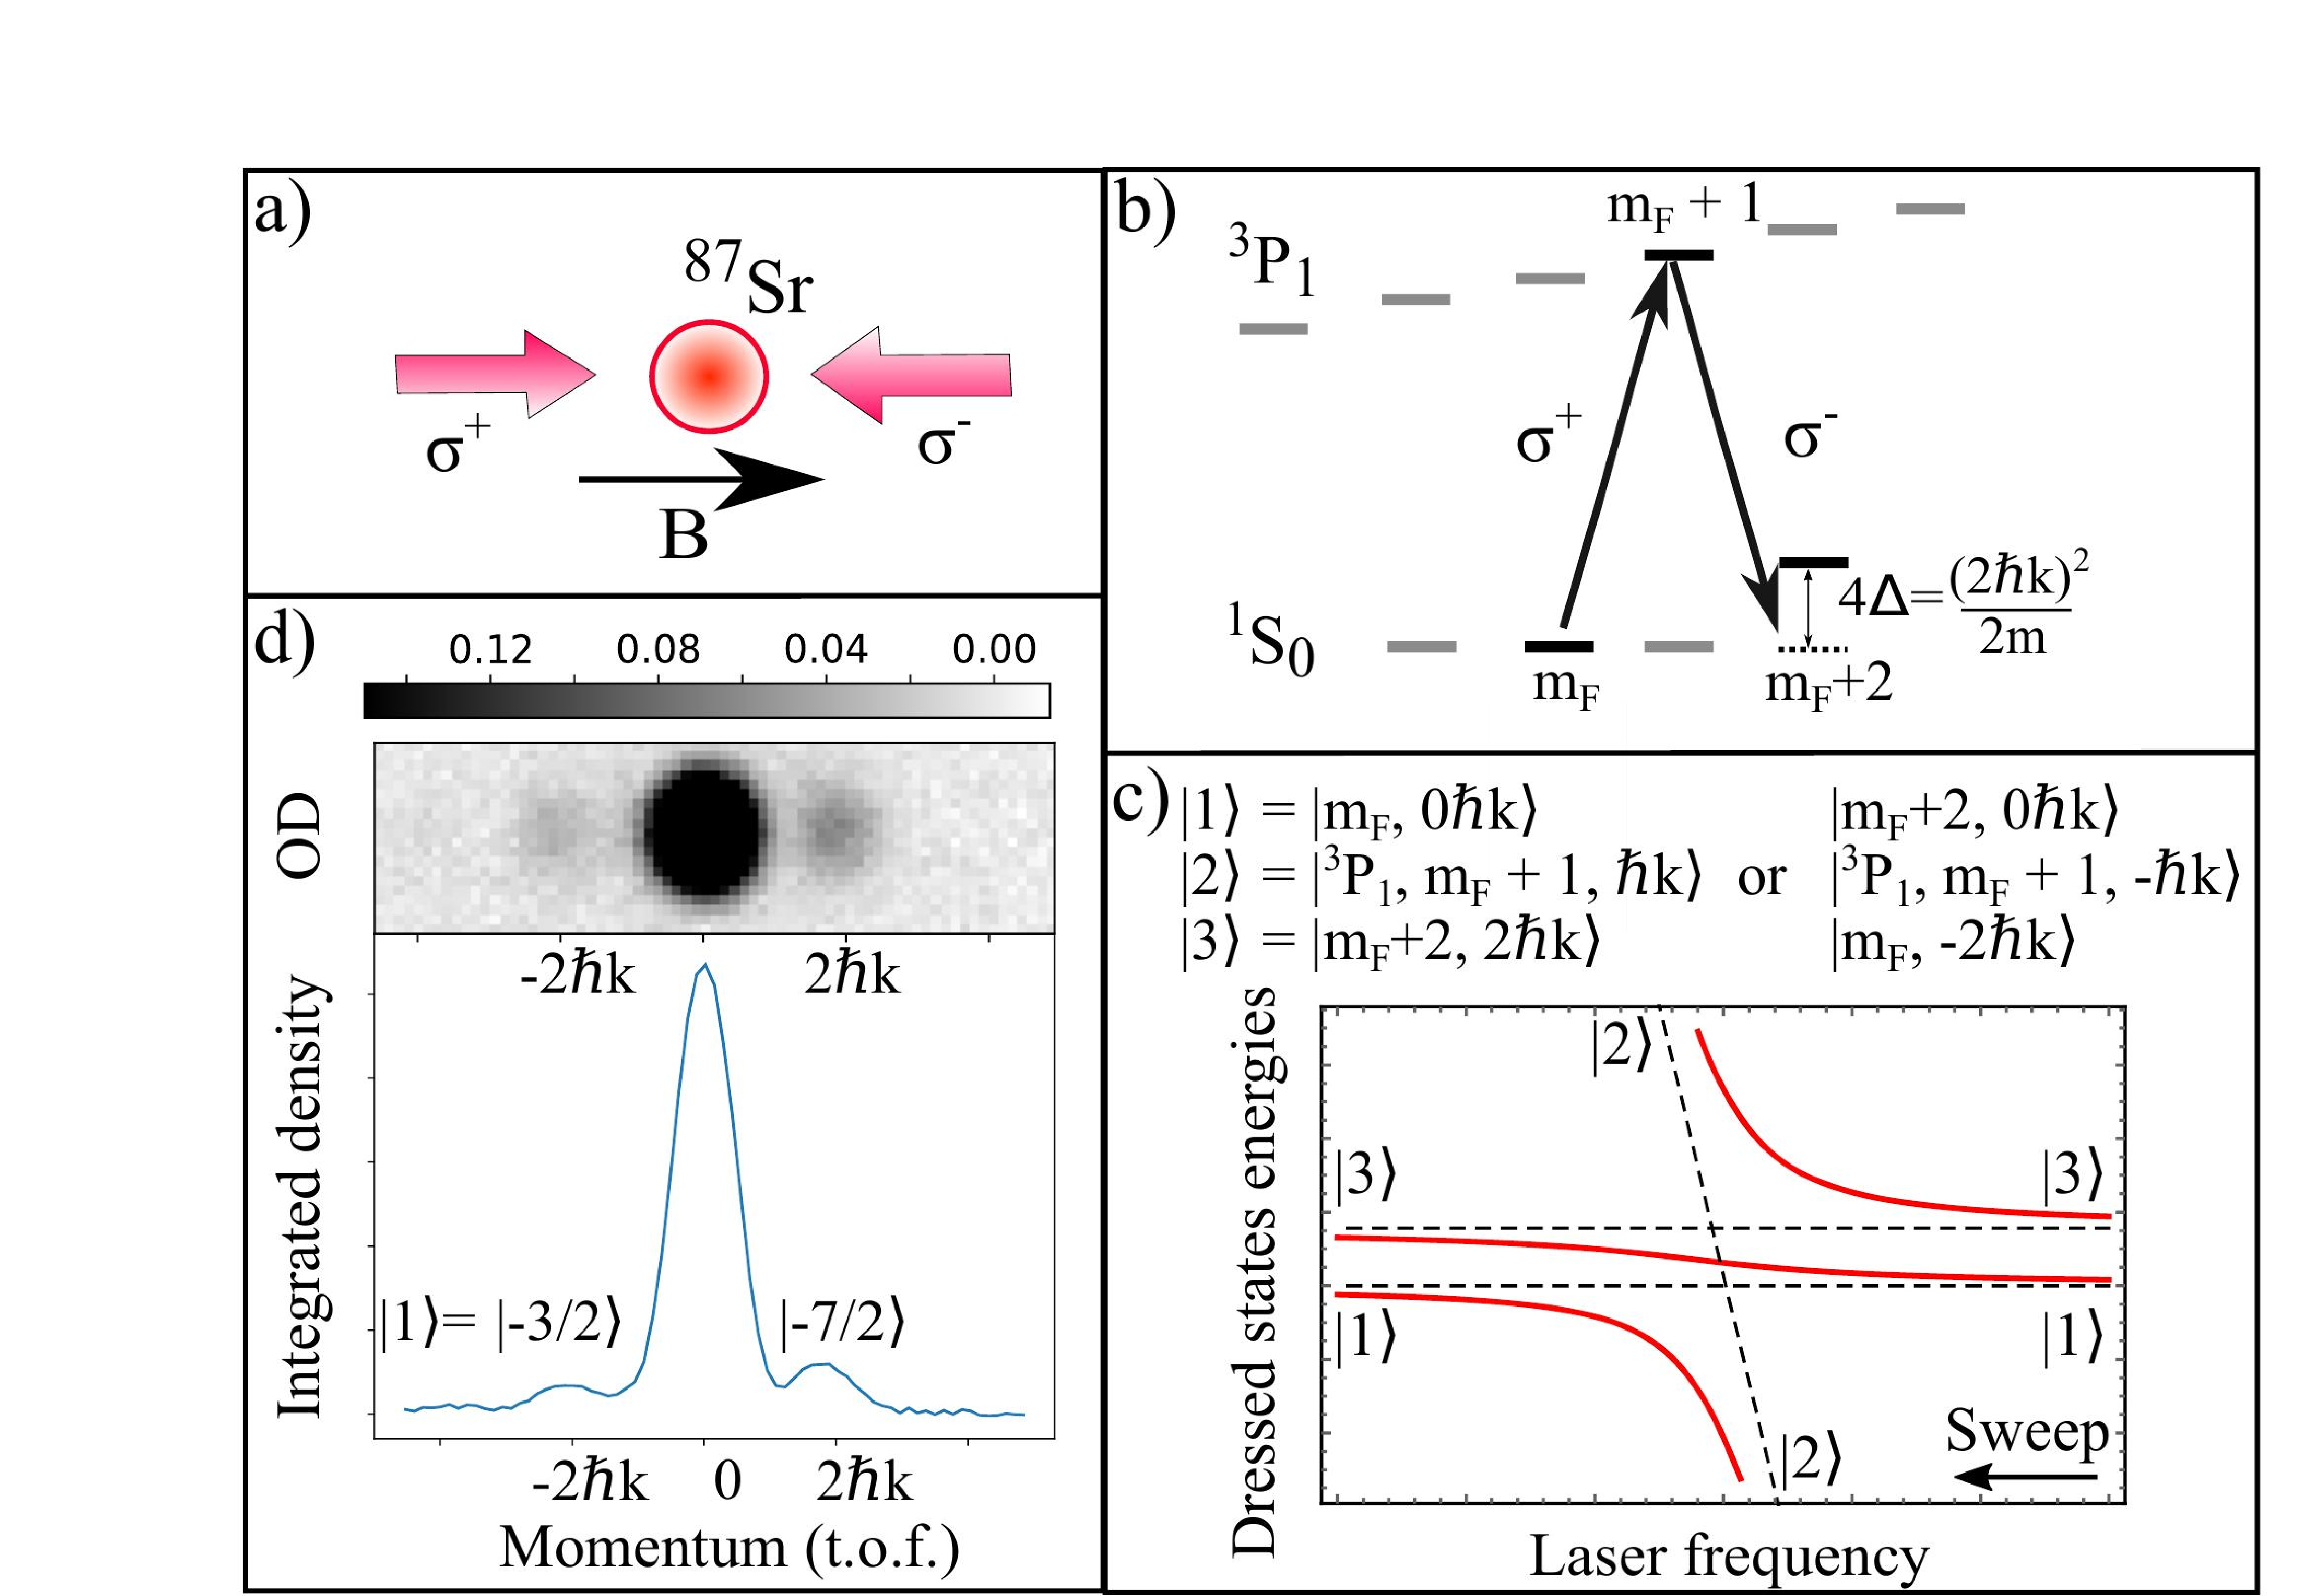
\includegraphics[width=1\linewidth]{Chapitres/Gas preparation and spin control/images/figure1_adiabatic_passage.pdf}
    \caption[Principle of spin-selective detection via coherent momentum transfer.]{Principle of spin-selective detection via coherent momentum transfer. (a) Counter-propagating beam geometry of the lasers used for the TLS and two-photon Raman scheme. (b) Energy levels scheme of the Raman process, with recoil energy shifting the $m_F+2$ level. (c) Avoided crossing due to the coupling of the states, necessiting adiabatic transfer. (d) Resulting TOF absorption image showing spatially separated spin components and the corresponding momentum distribution.}
    \label{fig:intro-spin-kick-scheme}
\end{figure}